\documentclass[corpo=12pt,twoside,tipotesi=magistrale,stile=classica]{toptesi}
\usepackage[english,italian]{babel}
\usepackage[utf8]{inputenc}
\usepackage[autostyle]{csquotes}
\usepackage[backend=biber]{biblatex}
\usepackage[]{hyperref}
\usepackage{lipsum}
\usepackage{comment}
\usepackage[disable]{todonotes}
\usepackage{listings}
\usepackage{color}
\usepackage{caption}
\usepackage{subcaption}

\definecolor{dkgreen}{rgb}{0,0.6,0}
\definecolor{gray}{rgb}{0.5,0.5,0.5}
\definecolor{mauve}{rgb}{0.58,0,0.82}

\lstset{
	frame=tb,
	aboveskip=3mm,
	belowskip=3mm,
	showstringspaces=false,
	columns=flexible,
	basicstyle={\small\ttfamily},
	numbers=none,
	numberstyle=\tiny\color{gray},
	keywordstyle=\color{blue},
	commentstyle=\color{dkgreen},
	stringstyle=\color{mauve},
	breaklines=true,
	breakatwhitespace=true,
	tabsize=3
}

\addbibresource{Bibliografia/bibliografia.bib}

\hypersetup{
	colorlinks=true,
	linkcolor=black,
	filecolor=magenta,      
	urlcolor=cyan,
}

\excludecomment{commento}
\excludecomment{idee}
\excludecomment{scaletta}


\includeonly{sommario,DescrizioneAutopilota/px4,Simulazioni/sitl}


\begin{document}

	\begin{frontespizio*}
		\ateneo{Politecnico di Torino}
		\logosede{polito}
		\CorsoDiLaureaIn{Laurea Magistrale in}
		\corsodilaurea{Ingegneria Aerospaziale}	
		\TesiDiLaurea{Tesi Magistrale}
		\titolo{Software in the loop simulations and Code generation for Unmanned Aerial systems}
		\AdvisorName{Relatore:}
		\relatore{Dott.ssa Elisa Capello}
		\CoAdvisorName{Co-Relatore}
		\secondorelatore{Ing. Davide Carminati}
		\sedutadilaurea{Dicembre 2020}
		\TitoloListaCandidati{Autore:}
		\candidato{Luigi Sante}
	\end{frontespizio*}

	\sommario
La tesi prevede lo sviluppo del software necessario per il governo di un velivolo a pilotaggio remoto, implementando diversi modelli di controllo e validando il controllore con simulazioni, in cui è stato considerato il software di bordo.

Data la complessità della generazione del software necessario alla guida e controllo dei velivoli di questo tipo, l'approccio più intuitivo, che permette la collaborazione tra diverse figure professionali quali programmatori, ingegneri aerospaziali e meccatronici, risulta essere sicuramente basata sull'utilizzo di una logica progettuale a modelli. Questo tipo di approccio permette di semplificare lo sviluppo del software, concentrando gli sforzi di chi si occupa della creazione dei modelli di controllo sugli aspetti effettivamente importanti della funzionalità di questi, lasciando la complessità della generazione di algoritmi e le relative basi di dati a chi ha maggiore competenza informatica, attraverso lo sviluppo degli strumenti che automatizzano la generazione del codice e la sua compilazione. 
Lo sviluppo del software effettuato in questo modo è accompagnato per ogni passaggio dalla corrispettiva fase di verifica: MIL (Model in the loop), SIL (Software in the loop), PIL (Prosessor in the loop), HIL (Hardware in the loop); aspetto derivato proprio dal classica metodologia di sviluppo del software utilizzante il modello denominato a V, e pienamente solidificato in molti settori industriali.

\'E stato scelto di utilizzare per l'implementazione dell'autopilota il dispositivo PixHawk con il relativo firmware PX4. Lo sviluppo del software avviene quindi specificatamente per questo sistema di prodotti e relativi firmware. Il codice è open-source, permettendo la possibilità di essere studiato e modificato. Il codice si trova ad uno stato abbastanza evoluto nello sviluppo, possedendo tutta una serie di funzionalità già sufficiente per gestire un velivolo a pilotaggio remoto. Nel caso però si voglia inserire un personale modello di guida e controllo o un nuovo stimatore, non sono previsti nativamente strumenti di modellazione, limitando lo sviluppo del software solo alle persone con una competenza informatica elevata, incrementando la complessità di progettazione stessa. In definitiva si ha difficoltà di creazione del codice sorgente partendo da un modello ,esistono comunque gli strumenti per verificare il codice tramite SIL (Software in the loop) e PIL (Prosessor in the loop).

In modo complementare all'utilizzo di PX4, si affianca l'utilizzo di un tool specifico per Simulink, chiamato "Embedded Coder Support Package
for PX4 Autopilots". Grazie a questo tool si permette la generazione del codice in modo automatico partendo dai modelli creati su Simulink e l'inserimento conforme del modulo prodotto all'interno del firmware e delle restanti funzionalità. Integrando quindi gli strumenti di compilazione presenti in PX4 si possono effettuare le simulazioni SIL (Software in the loop) e PIL (Prosessor in the loop), avvicinando lo sviluppo ad una approccio più industriale.

Per testare correttamente il funzionamento di un velivolo a pilotaggio remoto, occorre ricreare in un ambiente simulato il velivolo stesso e le interazioni principali con l'ambiente in cui opera. La scelta dell'ambiente simulato ricade nell'utilizzo di Gazebo. Come anticipato precedentemente la procedura di SIL (Software in the loop) è nativamente presente nel progetto di PX4. I simulatori selezionabili per questa fase di test sono svariati, il tool di Simulink però limita la scelta ad un simulatore esterno solamente, ovvero JMavSim. Attraverso una procedura particolare però si è reso possibile l'utilizzo di Gazebo, ambiente più versatile e completamente personalizzabile.

Sono stati creati due modelli di controllo delle diverse dinamiche del velivolo e successivamente alla corretta configurazione dei parametri dei controllori, sono stati messi a confronto attraverso simulazioni SIL (Software in the loop). Per quando riguarda il controllo di posizione è stato utilizzato un semplice controllore PID (Proportional Iintegral Derivative), mentre per il controllo di quota e di assetto, sono stati utilizzati rispettivamente un controllore PID e un controllore SMC (Sliding Mode Control). L'algoritmo di guida invece prevede la generazione della traiettoria con profili di velocità trapezoidali.

Non è invece stato possibile effettuare correttamente la simulazione PIL (Prosessor in the loop) a causa di alcuni problemi di comunicazione tra simulatore PixHawk. La trasmissione tra simulatore e autopilota avviene correttamente per quanto riguarda la gestione dei dati dei sensori, ciò non viene altrettanto per quanto riguarda i messaggi da fornire agli attuatori. Questo problema é probabilmente causato dalla differenza sostanziale che c'è tra l'applicazione generata dal tool di Simulink e la logica di base di PX4 nella gestione dei messaggi agli attuatori. Questo aspetto richiede ulteriori indagini in lavori futuri.

\begin{commento}
Inglese

The main purpose of this work is the development of the software necessary for the steering of a UAV (Unmanned Aerial Vehicle) with implementation of different control models and  the validation of the controller with software in the loop.

Given the complexity of the generation of the software necessary to guide and control UAVs (Unmanned Aerial Vehicle), the more intuitive approach, which allows collaboration between different professionals such as programmers, aerospace and mechatronics engineers, is certainly model based design. This type of approach makes it possible to simplify software development, concentrating the efforts the development of control models with focus on important aspects of their functionality, leaving the complexity of generating algorithms and related datastructure to those who have greater IT competence through the development of tools that automate the generation of the code and its compilation.
The software development carried out in this way is validated for each step by the corresponding verification phase: MIL (Model in the loop), SIL (Software in the loop), PIL (Prosessor in the loop), HIL (Hardware in the loop); derived from the classic software development V- model methodology, that is standard in many industrial sectors.

The implementation of the autopilot was made it on the PixHawk 4 device with the relative PX4 firmware. Therefore,the software development takes place specifically for these product systems and related firmware. The code is open-source, allowing the possibility to be studied and modified. The code is fully functional, possessing a whole series of features already sufficient to manage a remotely piloted aircraft. However, if you want to insert a personal GNC (Guidance , navigation and control) model or a new estimator, modeling tools not exist natively, limiting software development only to people with high IT (Information technology) skills, increasing the  overall design complexity itself. Ultimately, it is difficult to create the source code starting from a model, however there are tools included in che sources directory to verify the code through SIL (Software in the loop) and PIL (Prosessor in the loop).

MathWorks has made available a tool called "Embedded Coder Support Package
for PX4 Autopilots " that allows to compensate the aforementioned limitations. Thanks to this tool it is possible to generate the code automatically starting from the models created on Simulink and the insertion of the produced module into the firmware structure with the remaining useful functions. Therefore, integrating the compilation tools included in PX4, SIL (Software in the loop) and PIL (Prosessor in the loop) simulations can be performed, as a more industrial approach.

In order to properly test the operation of the UAV (Unmanned Aerial Vehicle), it is necessary to recreate in a simulated environment the aircraft itself and the main interactions with that. The choice of the simulated environment falls back on Gazebo. As previously mentioned, the SIL (Software in the loop) procedure is natively present in the PX4 project. The simulators that can be selected for this test phase are varied, the Simulink tool however limits the choice to an external simulator only that is JMavSim. However, through a particular procedure, it was possible to use Gazebo, a more versatile and customizable environment.

Two control models of the different dynamics of the aircraft were created and after the correct configuration of the controllers parameters, they were compared through SIL (Software in the loop) simulations. A simple PID (Proportional Iintegral Derivative) controller was used as position controller and a PID (Proportional Integral Derivative) controller and a SMC (Sliding Mode Control) controller respectively were used in order to attitude control. The GNC (Guidance, navigation and control) algorithm foresees a planning trajectory using trapezoidal velocity profile.

The PIL (Prosessor in the loop) simulation could not be performed correctly due to some communication problems between the PixHawk an the simulator. The transmission between the simulator and the autopilot takes place correctly as regards the management of sensor data, this was not the same as regards the messages to be provided to the actuators. This problem was probably caused by the substantial difference between the application generated by the Simulink tool and the basic logic of PX4 in managing messages to the actuators. This aspect requires further investigation in future work.

Abstract

The main purpose of this work is the development of the software necessary for the steering of a UAV (Unmanned Aerial Vehicle) with implementation of different control models and  the validation of the controller with software in the loop.
Given the complexity of the generation of the software necessary to guide and control UAVs (Unmanned Aerial Vehicle), the more intuitive approach, which allows collaboration between different professionals such as programmers, aerospace and mechatronics engineers, is certainly model based design.
The software development carried out in this way is validated for each step by the corresponding verification phase: MIL (Model in the loop), SIL (Software in the loop), PIL (Prosessor in the loop), HIL (Hardware in the loop); derived from the classic software development V- model methodology, that is standard in many industrial sectors.
The implementation of the autopilot was made it on the PixHawk 4 device with the relative PX4 open-source firmware. The code is fully functional, possessing a whole series of features already sufficient to manage a remotely piloted aircraft. However, if you want to insert a personal GNC (Guidance , navigation and control) model or a new estimator, modeling tools not exist natively, limiting software development only to people with high IT (Information technology) skills, increasing the  overall design complexity itself.
MathWorks has made available a tool called "Embedded Coder Support Package
for PX4 Autopilots " that allows to compensate the aforementioned limitations. Thanks to this tool it is possible to generate the code automatically starting from the models created on Simulink and the insertion of the produced module into the firmware structure with the remaining useful functions. Therefore, integrating the compilation tools included in PX4, SIL (Software in the loop) and PIL (Prosessor in the loop) simulations can be performed, as a more industrial approach.
The choice of the simulated environment falls back on Gazebo.
Two control models of the different dynamics of the aircraft were created and after the correct configuration of the controllers parameters, they were compared through SIL (Software in the loop) simulations. A simple PID (Proportional Iintegral Derivative) controller was used as position controller and a PID (Proportional Integral Derivative) controller and a SMC (Sliding Mode Control) controller respectively were used in order to attitude control. The GNC (Guidance, navigation and control) algorithm foresees a planning trajectory using trapezoidal velocity profile.
The PIL (Prosessor in the loop) simulation could not be performed correctly due to some communication problems between the PixHawk an the simulator. The transmission between the simulator and the autopilot takes place correctly as regards the management of sensor data, this was not the same as regards the messages to be provided to the actuators. This problem was probably caused by the substantial difference between the application generated by the Simulink tool and the basic logic of PX4 in managing messages to the actuators. This aspect requires further investigation in future work.

\end{commento}

	\ringraziamenti
	
	\tableofcontents
%	\listoftables
	\listoffigures
	
	\mainmatter
	
	\chapter{Introduzione}
La tesi prevede lo sviluppo del software necessario per il governo di un velivolo a pilotaggio remoto, implementando diversi modelli di controllo e validando il controllore con diverse simulazioni.

Data la complessità della generazione del software necessario alla guida e controllo dei velivoli di questo tipo, l'approccio più intuitivo, che permette la collaborazione tra diverse figure professionali quali programmatori, ingegneri aerospaziali e meccatronici, risulta essere sicuramente basata sull'utilizzo di una logica progettuale a modelli. Questo tipo di approccio permette di semplificare lo sviluppo del software, concentrando gli sforzi di chi si occupa della creazione dei modelli di controllo sugli aspetti effettivamente importanti della funzionalità di questi, lasciando la complessità della generazione di algoritmi e le relative basi di dati a chi ha maggiore competenza informatica, attraverso lo sviluppo degli strumenti che automatizzano la generazione del codice e la sua compilazione. 
Lo sviluppo del software effettuato in questo modo è accompagnato per ogni passaggio dalla corrispettiva fase di verifica: MIL, SIL, PIL, HIL; aspetto derivato proprio dal classica metodologia di sviluppo del software utilizzante il modello denominato a V, e pienamente solidificato in molti settori industriali.

\'E stato scelto di utilizzare per l'implementazione dell'autopilota il dispositivo PixHawk con il relativo firmware PX4. Lo sviluppo del software avviene quindi specificatamente per questo ecosistema di prodotti e relativi firmware. Il codice è open-source, permettendo la possibilità di essere studiato e modificato. Il codice si trova ad uno stato abbastanza evoluto nello sviluppo, possedendo tutta una serie di funzionalità già sufficiente per gestire un velivolo a pilotaggio remoto. Nel caso però si voglia inserire un personale modello di guida e controllo o di un nuovo stimatore, non sono previsti nativamente strumenti di modellazione, limitando lo sviluppo del software solo alle persone con una competenza informatica alta, incrementando la complessità di progettazione stessa. In definitiva si ha difficoltà di creazione del codice sorgente partendo da un modello ,esistono comunque gli strumenti per verificare il codice tramite SIL e PIL.

In modo complementare all'utilizzo di PX4, si affianca l'utilizzo di un tool specifico per Simulink, chiamato "Embedded Coder Support Package
for PX4 Autopilots". Grazie a questo tool si permette la generazione del codice in modo automatico partendo dai modelli creati su Simulink e l'inserimento conforme del modulo prodotto all'interno del firmware e delle restanti funzionalità. Integrando quindi gli strumenti di compilazione presenti in PX4 si possono effettuare le simulazioni SIL e PIL, avvicinando lo sviluppo ad una approccio più industriale.

Per testare correttamente il funzionamento di un velivolo a pilotaggio remoto, occorre ricreare in un ambiente simulato il velivolo stesso e le interazioni principali con l'ambiente in cui opera. La scelta dell'ambiente simulato ricade nell'utilizzo di Gazebo. Come anticipato precedentemente la procedura di SIL è nativamente presente nel progetto di PX4. I simulatori selezionabili per questa fase di test sono svariati, il tool di Simulink però limita la scelta ad un simulatore esterno solamente, ovvero JMavSim. Attraverso una procedura particolare però si è reso possibile l'utilizzo di Gazebo, ambiente più versatile e completamente personalizzabile.

Sono stati creati due modelli di controllo delle diverse dinamiche del velivolo e successivamente alla corretta configurazione dei parametri dei controllori, sono stati messi a confronto attraverso simulazioni SIL. Per quando riguarda il controllo di posizione è stato utilizzato un semplice controllore PID, mentre per il controllo di quota e di assetto, sono stati utilizzati rispettivamente un controllore PID e un controllore SMC. 
\todo{Che tipo di algoritmo di guida è stato utilizzato?}

Non è invece stato possibile effettuare correttamente la simulazione PIL a causa di alcuni problemi di comunicazione tra simulatore PixHawk. La trasmissione tra simulatore e autopilota avviene correttamente per quanto riguarda la gestione dei dati dei sensori, ciò non viene altrettanto per quanto riguarda i messaggi da fornire agli attuatori. Questo problema é probabilmente causato dalla differenza sostanziale che c'è tra l'applicazione generata dal tool di Simulink e la logica di base di PX4 nella gestione dei messaggi agli attuatori. Questo aspetto richiede ulteriori indagini in lavori futuri.	
	
	%\chapter{Sistema Quadrirotore}
	\chapter{Sistema Quadrirotore}
Il capitolo è incentrato sulla descrizione del modello matematico del sistema quadricottero con le relative dinamiche, leggi di guida e leggi di controllo possibili da implementare.
\section{Modello matematico}
\todo[inline]{Principi di funzionamento}
\todo[inline]{il sistema di riferimento}
\todo[inline]{Figura della configurazione del drone
tipo di azionamento base}
\todo[inline]{Definizione degli operatori necessari a descrivere il modello base del drone}

	\section{Leggi di controllo}
In questa sezione verranno accennati diversi modelli di controlli utilizzati odiernamente per controllare i quadricotteri, \cite{ZuluAndrew2014ARoC}, \cite{KimJinho2020ACSo}, \cite{PID_vs_LQ}, \cite{G_inf}. Questi si possono classificare in tre categorie come in Figura (\ref{fig:categoriecontrolli}).
\begin{figure}
	\centering
	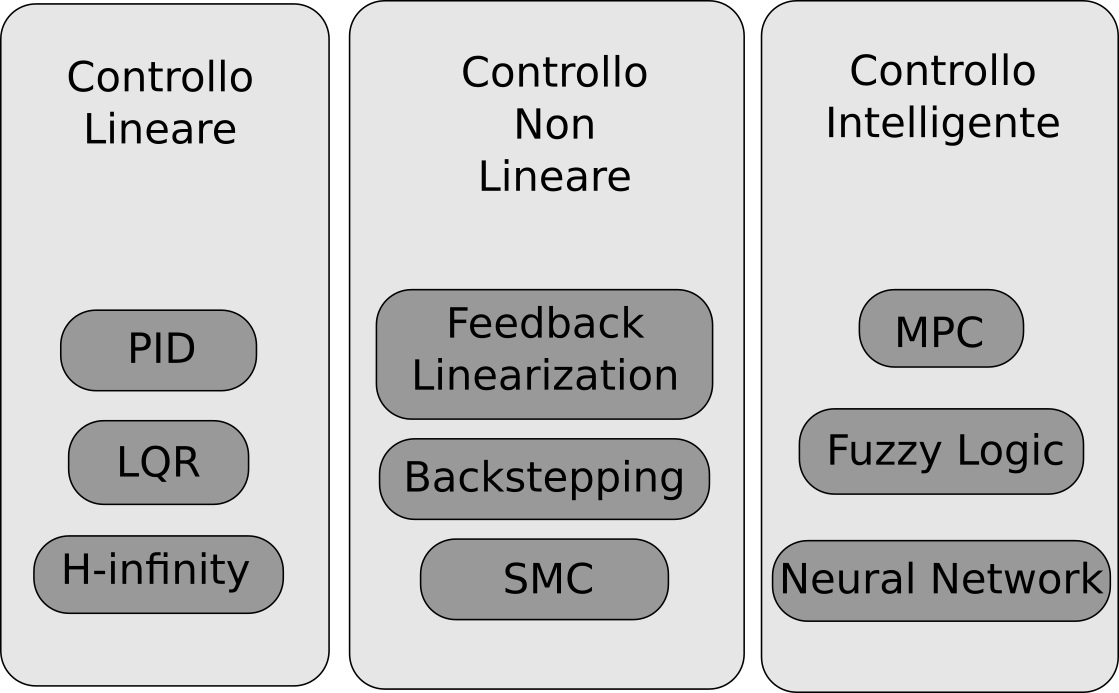
\includegraphics[width=0.6\textwidth]{SistemaQuadrirotore/Figure/Classificazione}
	\caption{Classificazione dei tipi di controllori maggiormente utilizzati \cite{KimJinho2020ACSo}}
	\label{fig:categoriecontrolli}
\end{figure}

\todo[inline]{Assunzioni, formule e citazioni per ogni controllore soprattutto PID e SMC}


\subsection{Controllori Lineari}
\subsubsection{Controllore Proportional-Integral-Derivative Controller (PID)}
Il controllore PID è molto utilizzato in diverse applicazioni, la sua semplicità e facilità di impostazione dei parametri lo rende molto rapido da implementare e relativamente robusto. Inoltre non è necessario avere la misura dello stato completo del sistema da controllare, semplificando eventualmente la determinazione di questo. Il principale problema risiede nella risposta alle eventuali non linearità presenti nel modello del sistema controllato o nella realtà.
Si definisce un errore di misurazione $e(t)$ come la differenza tra il valore atteso $x(t)_{ref}$ e il valore misurato nel sistema $x(t)$ di un qualunque elemento del vettore di stato : $e(t)=x(t)_{ref}-x(t)$. Attraverso la misurazione dell'errore, applicando l'equazione integro differenziale (\ref{eq:SistemaQuadrirotore_PIDErrore}), si determina il comando da attuare sul sistema \cite{pid-controllers-theory}.
\begin{equation}\label{eq:SistemaQuadrirotore_PIDErrore}
	u(t) = k_p e(t) + k_i \int_0^t e(\tau) d\tau + k_d \frac{d e(t)}{d t}
\end{equation}
Il nome del controllore deriva proprio dalla combinazione di questi tre aspetti presi in considerazione per valutare il comando da attuare.
Nell'equazione (\ref{eq:SistemaQuadrirotore_PIDErrore}) sono presenti i tre parametri: $k_p$, $k_i$ e $k_d$.
L'effetto del guadagno proporzionale $k_p$ è quello di ridurre l'errore in modo proporzionale allo stesso. Più l'errore è grande più sarà importante l'intervento del controllore per ridurlo. Un guadagno troppo alto però può provocare un grande superamento del segnale di riferimento causando un overshoot e l'amplificazione delle oscillazioni nella fase di assestamento.
L'effetto $k_i$ è quello ridurre l'errore stazionario terminata la fase di assestamento. Il solo utilizzo della componente proporzionale non è infatti sufficiente per ridurre anche l'errore stazionario, definito come il valore assunto dall'errore trascorso un tempo sufficientemente lungo. Con il solo effetto proporzionale l'errore stazionario si assesta ad un valore finito, il valore integrale dell'errore tende ad aumentare nel tempo se questo on viene annullato, determinando una retroazione integrale che tende a ridurlo.
La derivata dell'errore è invece utile a prevedere il comportamento di questo nel tempo, anticipando l'effetto del proporzionale. Tenendo conto del suo andamento, attraverso il valore di $k_d$, si può ridurre il picco generato da un guadagno alto dell'effetto proporzionale. Questo contributo però va usato con cautela perché amplificare il rumore presente nelle misurazioni.
Il settaggio di questi parametri viene fatta impostando inizialmente solo il valore di $k_p$. Successivamente per ridurre il valore dell'errore stazionario viene aumentato il guadagno $k_i$. Modificando il valore $k_d$ si può ottenere un miglioramento in termini di risposta del sistema, rendendola più stabile. Il processo è iterativo fino ad ottenere una risposta desiderata.


\begin{figure}
	\centering
	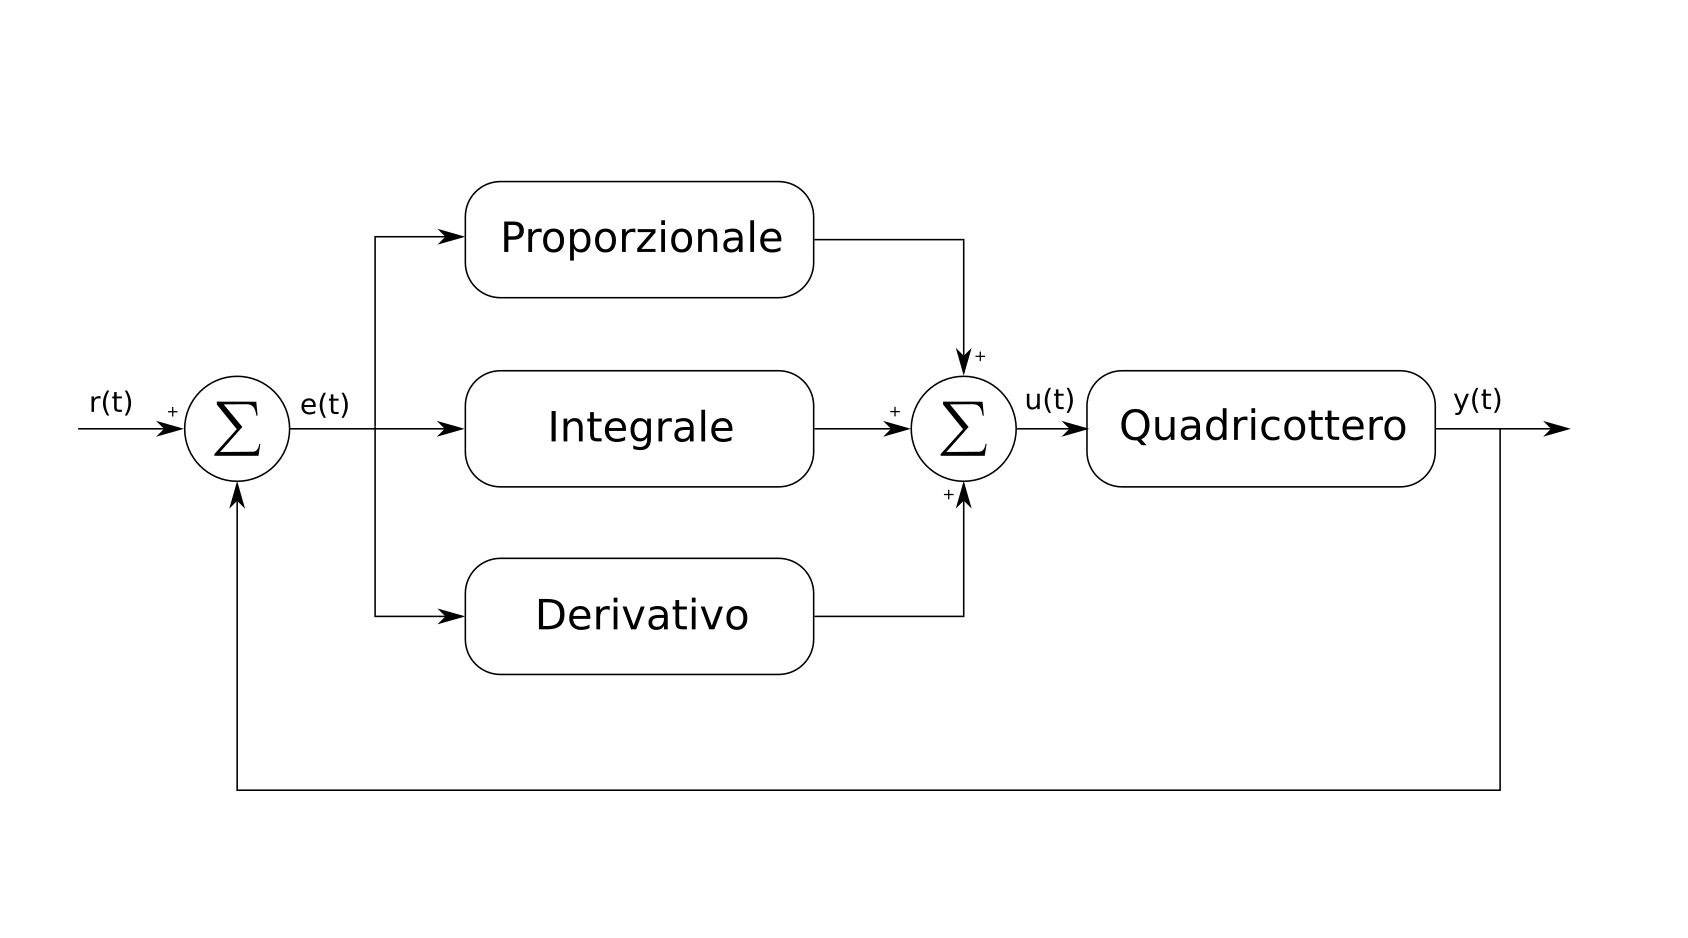
\includegraphics[width=0.6\textwidth]{SistemaQuadrirotore/Figure/PID}
	\caption{Schema di applicazione del controllore PID}
\end{figure}

\subsubsection{Controllore Linear Quadratic Regulator (LQR)}
Con la minimizzazione della funzione di costo espressa nella equazione (\ref{eq:SistemaQuadrirotore_LQRCosto}), si ottiene una matrice di guadagni con la quale si applica il controllo in retroazione \cite{bibid}. A differenza del PID, questo tipo di controllo prevede di avere tutto il vettore di stato a disposizione. Per questo motivo viene accompagnato spesso da un Linear Quadratic Estimator (LQE) ed un filtro di Kalman, con lo scopo di determinare dalle misurazioni dei sensori lo stato del sistema. Il metodo utilizzato per determinare la matrice dei guadagni è un aspetto molto importante, inoltre è necessario modellare in modo molto preciso il sistema controllato per evitare di trovare una soluzione poco soddisfacente. Questo tipo di controllo può essere specializzato per ottenere una soluzione ottima di risparmio della batteria \cite{KoksalN2018ALQA}, risultando però poco robusti \cite{ZuluAndrew2014ARoC}.

\begin{equation}\label{eq:SistemaQuadrirotore_LQRCosto}
	J = \int_{0}^{t} \left[e(t)^T \mathbf{Q}\right]
\end{equation}

\begin{figure}
	\centering
	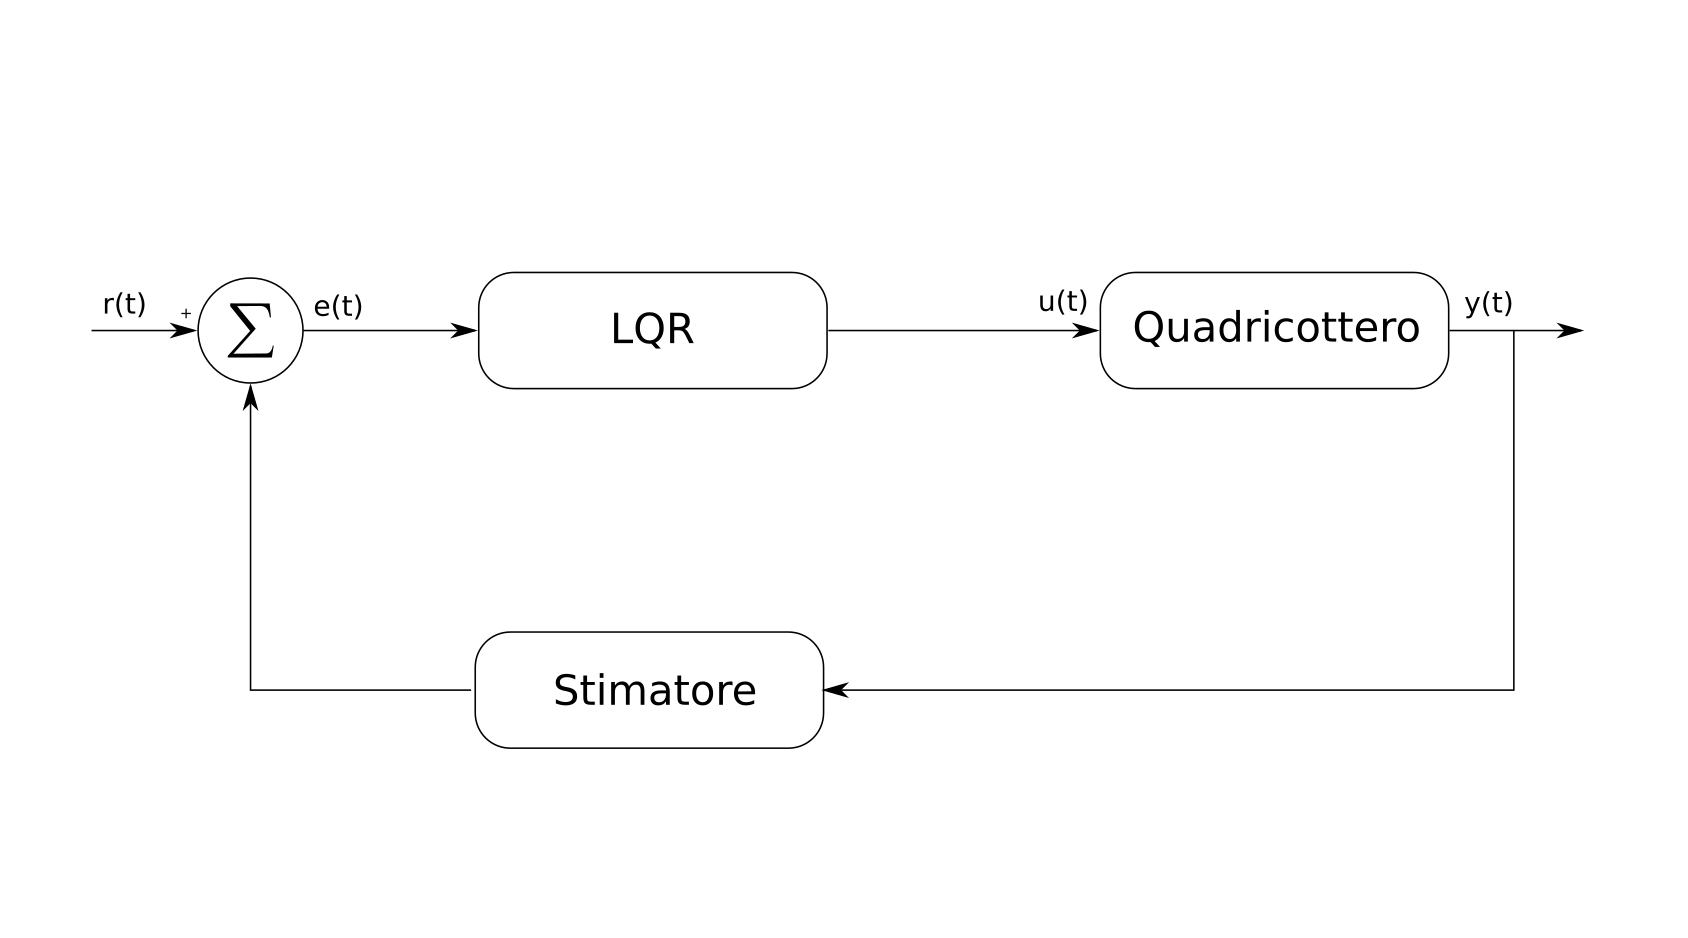
\includegraphics[width=0.6\textwidth]{SistemaQuadrirotore/Figure/LQR}
	\caption{Schema di applicazione del controllore LQR}
\end{figure}
 

\subsubsection{Controllore $H_\infty$}

Il controllore $H_\infty$ si ottiene esprimendo la soluzione del controllo attraverso una formulazione matematica, prende il nome dallo spazio matematico in cui ha luogo l'ottimizzazione, ovvero lo spazio di Hardy. Il problema principale di questo approccio è la complessità analitica che risiede nell'ottimizzazione stessa. Il sistema così trovato però ha il vantaggio di essere di più facile implementazione su sistemi multi-variabili. 

\subsection{Controllori non lineari}

\subsubsection{Controllore con Feedback Linearization}

Questo tipo di controllore viene utilizzato comunemente. La logica di funzionamento prevede di utilizzare un controllo lineare prestante. Introducendo una mappatura dell'ingresso al sistema, attuando di fatto un cambiamento di variabili di controllo, si fa in modo che il sistema lineare sia in grado di controllare il sistema controllato efficacemente. Il controllo lineare comanda quindi un sistema linearizzato equivalente al sistema non lineare. Questo tipo di approccio ha lo svantaggio però di essere molto sensibile alle incertezze e i rumori dei sensori, fattore che ne inficia la robustezza.

\begin{figure}
	\centering
	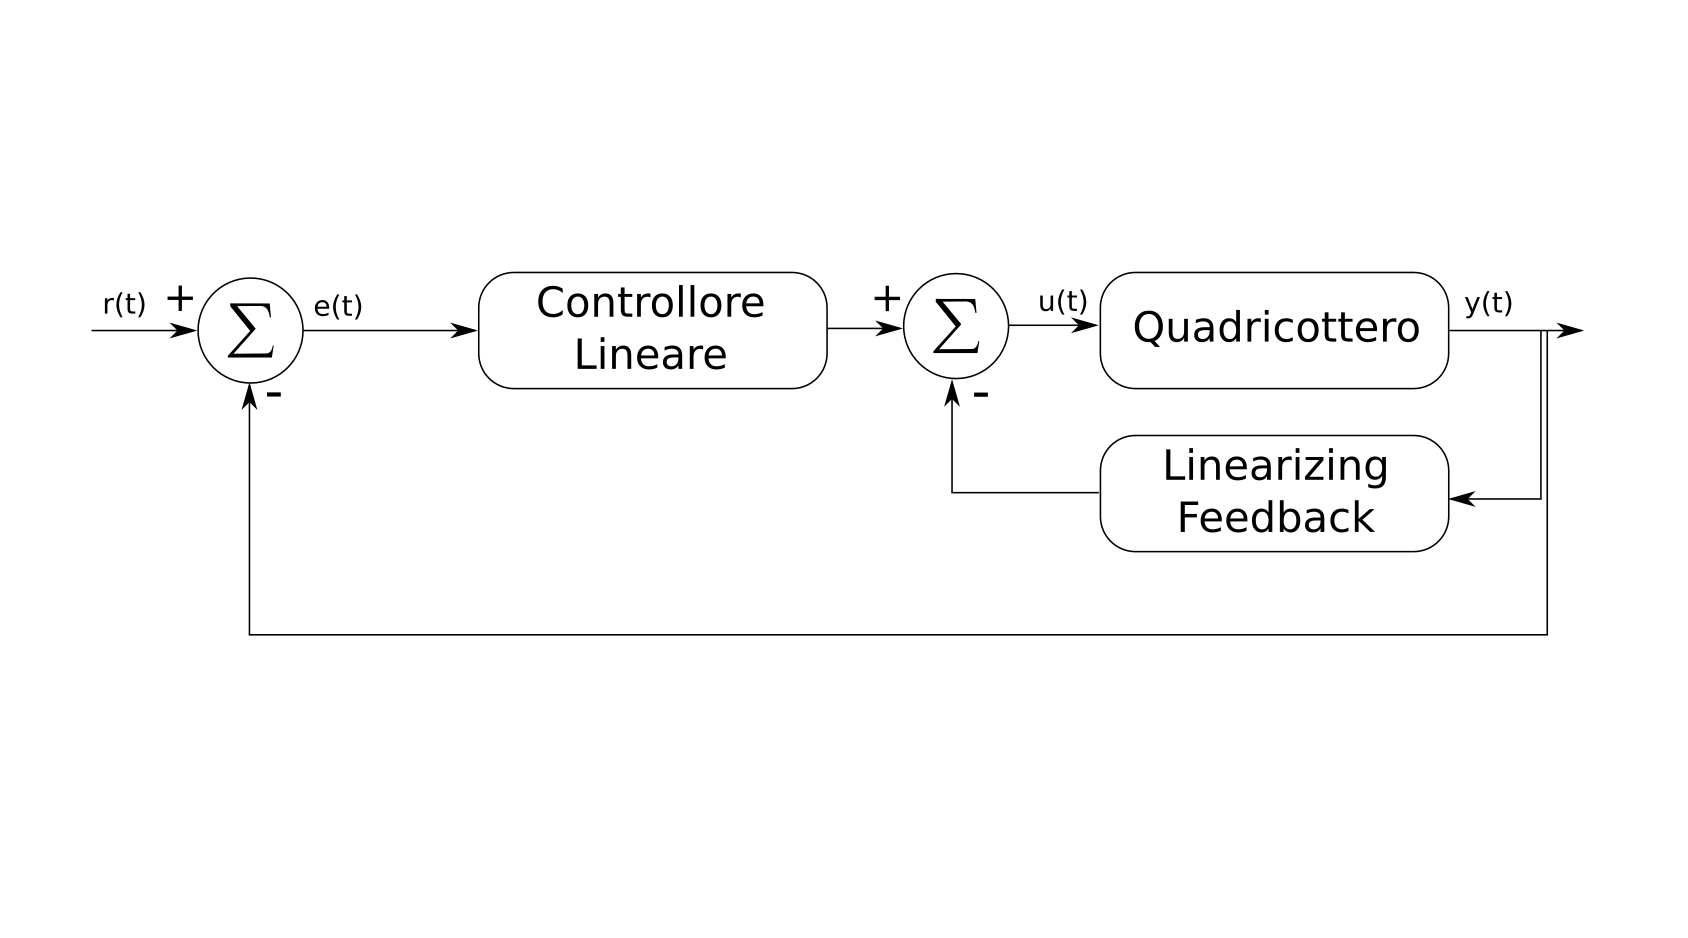
\includegraphics[width=0.6\textwidth]{SistemaQuadrirotore/Figure/FLP}
	\caption{Schema di applicazione del controllore con Feedback Linearization}
\end{figure}

\subsubsection{Controllore con Backstepping}

Si basa su di un algoritmo ricorsivo che segmenta il controllore in sottoparti, stabilizzando queste parti in modo progressivo. Questo tipo di controllore ha una procedura di convergenza molto rapida. Il suo difetto maggiore è la poca robustezza. Per poter migliorare la risposta può essere aggiunto un integratore con l'obbiettivo di ridurre l'errore stazionario.


\subsubsection{Controllore Sliding Mode Control (SMC)}

Questo tipo di controllo prevede di utilizzare un segnale di comando discontinuo, la legge di controllo non è quindi continua nel tempo. Questo sistema risulta essere molto preciso e robusto, come verrà mostrato nelle simulazioni successive. A causa della discontinuità introdotta si può  osservare il fenomeno di chattering, che ha come effetto secondario l'aumento dell'utilizzo degli attuatori, ovvero un maggior consumo di batteria. Questo effetto può essere mediato applicando alcuni filtri in uscita dal controllore, che mediano le discontinuità. Il controllo basa il funzionamento sulla definizione di una superfice di sliding definita dallo stato del sistema, una volta portato su questa superficie attraverso il segnale discontinuo il controllore mantiene le oscillazioni nei dintorni di questa. Questo tipo di controllore è molto robusto e si comporta bene in presenza di rumore ed incertezze come l'effetto suolo.

\begin{figure}
	\centering
	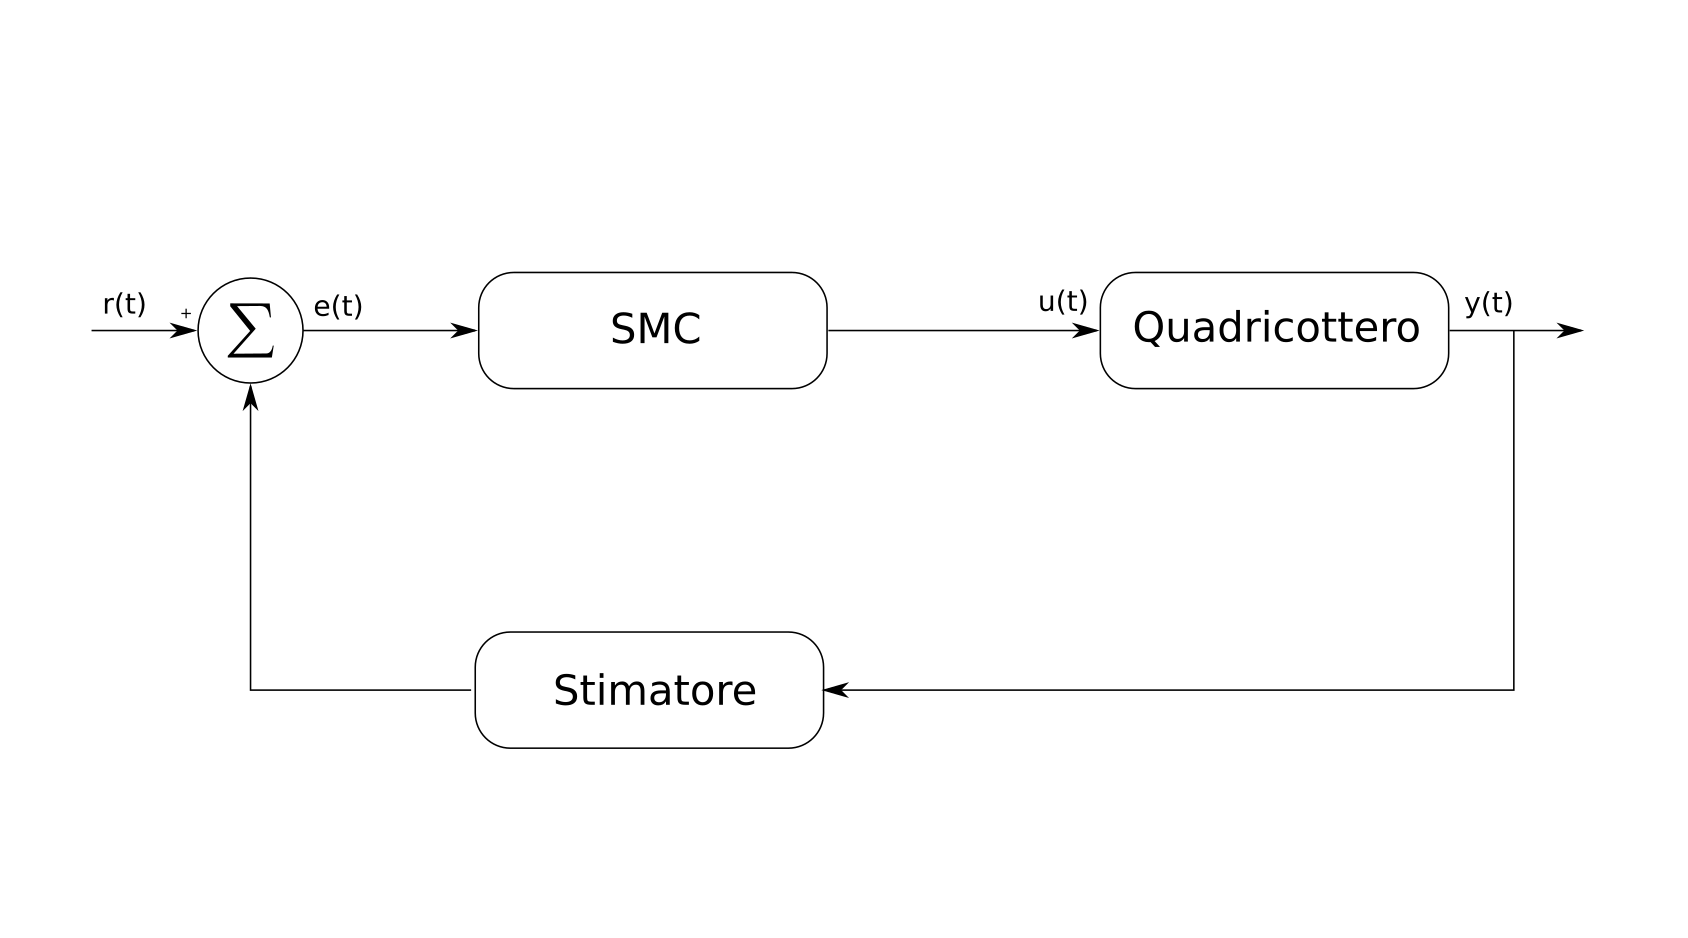
\includegraphics[width=0.6\textwidth]{SistemaQuadrirotore/Figure/SMC}
	\caption{Schema di applicazione del controllore SMC}
\end{figure}

\subsection{Controllori intelligenti}

\subsubsection{Controllore con Modello predittivo (MPC)}

Questo tipo di controllo si basa sulla previsione dello stato e del comando che verrà attuato seguendo dei modelli previsionali e stimatori. Molto utile se si vuole evitare di superare alcune imposizioni specifiche (forzare input e output in determinati contorni).
E' necessario un buon stimatore. Il controllore è in grado di reagire efficacemente in presenza di guasti ai motori.

\begin{figure}
	\centering
	
\includegraphics[width=0.6\textwidth]{SistemaQuadrirotore/Figure/MPC}
	\caption{Schema di applicazione del controllore MPC}
\end{figure}

\subsubsection{Controllore con logica Fuzzy}

Questo tipo di controllo si basa sulla presenza di stati logici non binari, range di valori  . Una serie di verifiche di condizioni soddisfatte con eventuali azionamenti specifici seguendo un algoritmo. Ad ogni passaggio il segnale di uscita viene determinando tenendo conto di diversi step per poter essere mandato al velivolo controllato. Non richiedono una conoscenza completa del sistema.

\begin{figure}
	\centering
	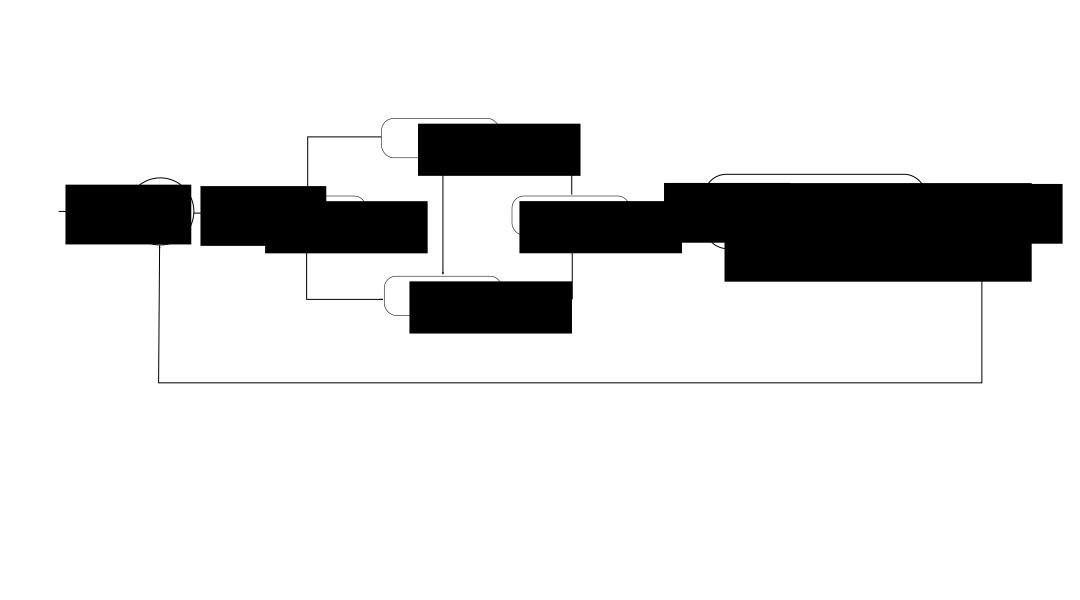
\includegraphics[width=0.8\textwidth]{SistemaQuadrirotore/Figure/Fuzzy}
	\caption{Schema di applicazione del controllore Fuzzy}
\end{figure}

\subsubsection{Controllore con Neural Network}

Si utilizza una rete neurale formata da diversi layer con la quale attraverso una fase di addestramento si ottiene un sistema di controllo. La rete è formata da neuroni collegati attraverso dei collegamenti pesati. Il vantaggio di questo metodo di controllo è la capacità di avere risultati migliori rispetto ai normali controlli lineari senza dover necessariamente conoscere la dinamica del quadrirotore e i suoi parametri.

\begin{figure}
	\centering
	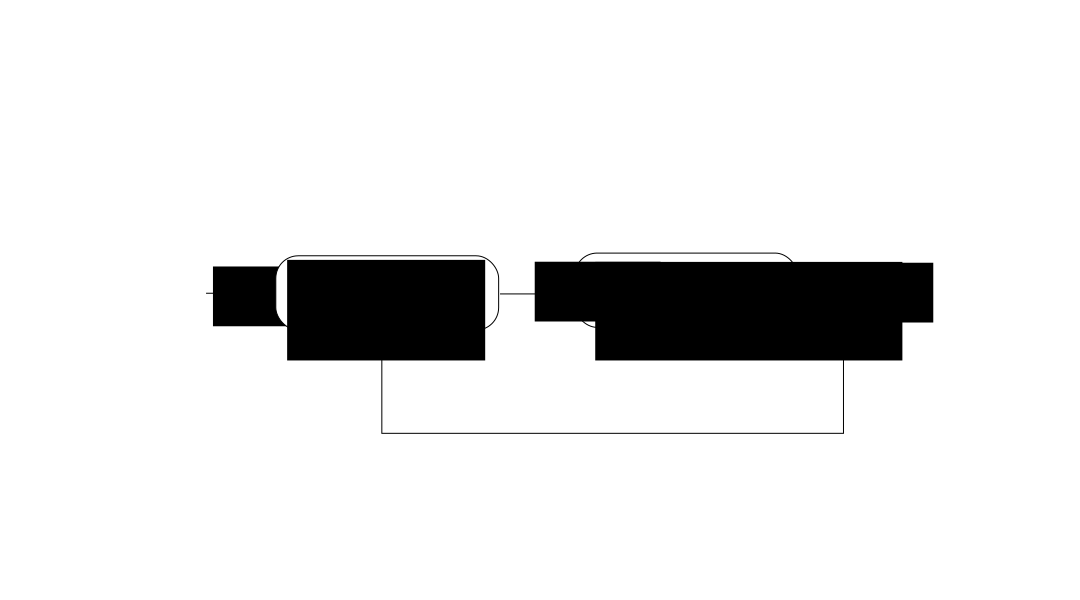
\includegraphics[width=0.6\textwidth]{SistemaQuadrirotore/Figure/NN}
	\caption{Schema di applicazione del controllore con Neural Network}
\end{figure}

	\section{Algoritmi di guida}

%\begin{idee}
%	\cite{ElikerKaram2018AOPf}
%	\cite{baseTesi}
%	\cite{Mendoza-SotoJoséLuis2018Cgpc}
%	\cite{PathPlannigOverview}
%	
%	
%	\cite{YangLiang2016SoR3} : 
%	
%	La necessità è quella di avere autonomia nello spostamento senza l'intervento dell'uomo, determinando autonomamente il percorso da seguire.
%	Tra gli obbiettivi di pianificazione del percorso c'è anche quello di evitare gli ostacoli possibili per questioni di sicurezza.
%	Nel contesto degli UAV il problema è un problema tridimensionale.
%	
%	La soluzione a questo tipo di problema è estremamente complessa.
%	
%	Si può suddividere il problema in 2 parti fondamentali:
%	
%	1. Percezione e modellazione dell'ambiente
%	2. Applicazione dell'algoritmo di pianificazione
%	
%	Non è necessario però che la pianificazione si sempre accompagnata da una ottimizazione, alcune volte basta che questa colleghi i due punti nello spazio.
%	Si distingue in pianificazione del persorso e pianificazione del percorso ottimo se si vuole ottimizzare una certa funzione di costo oppure no.
%	
%	Sussiste una differenza tra pianificazione del percorso e della traiettoria. La pianificazione del percorso cerca solo un a curva o una sequenza di curve che colleghino due punti nello spazio, mentre la pianificazione della traiettoria prevede di determinare anche come questa debba essere percorsa, descrivendo in modo cinematico e dinamico, attraverso la valutazione di questi nella ricerca della soluzione.
%	
%	Si possono classificare gli algoritmi di pianificazione dei percorsi in 5 categorie.
%	
%	1. Algoritmi basati sul campionamento:
%		Questi algoritmi richiedono la conoscenza a priori di informazioni sull'ambiente e una rappresentazione matematica di questo. Si prevede di dividere l'ambiente in nodi o celle o altre forme. Avviene poi una ricerca attraverso una ricerca casuale. Questa categoria si può suddividere a sua volta in altre 2 categorie : attive e passive. Attive  si intende algoritmi che esploraro rapidamente in modo casuale per trovare il percorso migliore. Passivi algoritmi che si occupano di cercare la soluzione da percorsi già presenti come su di una mappa.
%		Tra gli attivi si parla di Rapidly Exploring Random Tree (RRT). Si generano nodi casualmente nello spazio cercando di raggiungere il punto obbiettivo. L'algoritmo ha il problema però di essere molto lento se l'ambiente è disordinato per trovare la soluzione.
%		Dinamic Domain RRT (DDRRT) : questa evoluzione attraverso l'introduzione di sfere permette di velocizzare l'esplorazione dell'ambiente superando in parte la limitazione della versione RRT.
%		Rapidly Exploring Random Graph (RRG) : Per migliorare la soluzione ottenuta attraverso RRT e DDRRT viene introdotta una struttura dati che assiste l'esplorazione. Attraverso questo approccio nuovi collegamenti vengono fatti durante l'esplorazione per avere una soluzione migliorata. Ulteriore miglioramento può essere fatto utilizzando RRT-Star (RRT*) una versione in cui vengono eliminati i percorsi che si sono ottenuti e che probabilmente non sono ottimali , raffinando invece le connessioni che lo sono. In questo modo si ottiene una soluzione ottimizzata al prezzo però di non poter generare più percorsi contemporaneamente e un costo computazionale maggiore.
%		Probabilistic Road Map (PRM) genera i nodi in modo da avere un collegamento tra i due punti. Considera differenti scelte dal set di soluzioni che si possono trovare e attraverso un algoritmo di ricerca testa la soluzione per discriminare la migliore.
%		Vornoi: Attraverso l'uso dei digrammi di Voronoi si determinano i nodi e le connessioni per generare il percorso. Il vantaggio è che in questo approccio la minima distanza con gli ostacoli è sempre la stessa. Si continua a suddividere l'ambiente fino a quando si ottiene collegamento tra tutti i canali. Non è in grado di generare contemporaneamente il migliore percorso , per sopperire a questa limitazione è necessario utilizzare un algoritmo di ricerca per trovare la soluzione migliore.
%		Algoritmo basato su energia potenziale. Viene considerata una funzione potenziale attraverso interazione tra spazio percorribile e non, da questo si determina il percorso, è molto facile da implementare e ha un costo computazionale basso, ha però il problema di presentare minimi locali e punti di ristagno , limitazione però facilmente superabile in diversi modi.
%		Riassumendo questi approcci si basano sull'esplorazione delle possibili soluzioni e la successiva valutazione per migliorare la forma ottenuta. L'algoritmo si applica in modo indipendente all'ambiente specifico perché concettualmente separato avendo la capacità di determinare le collisioni in modo autonomo se nella ricerca avviene.
%	
%		
%	2. Algoritmi basati sui nodi
%		Questi algoritmi sono basati sull'utilizzo di nodi appartenenti ad un grafo scomposto, ricercando in mappe già pronte.
%		Algoritmo di Dijkstra.l Conoscendo già un grafo in cui gli archi e i nodi sono stati pesati , si attua una ricerca per ridurre la funzione di costo. Partendo quindi dai nodi si genera il grafo con i pesi e poi si applica l'algoritmo. Un evoluzione di questo algoritmo è A-Star (A*). Indroducendo una stima euristica del costo durante il processo di ricerca permetta una più veloce velocità di convergenza. Per applicazioni con ostacoli dinamici dsi utilizza una versione modificata denominata D-Star (D*) che prevede di modificare i pesi nel grafo in funzione della configurazione degli ostacoli. Questo tipo di approccio però è limitativo in termini di soluzioni a causa della chiara incompletezza della struttura di configurazioni nell'ambiente. Di fatto si parla solamente di un algoritmo di ricerca no è in grado di generare un percorso ma solo una configurazione di sotto-percorsi già precostituiti.
%		
%	3. Algoritmi basati su modelli matematici
%		Questi metodi modellano l'ambiente  e il sistema e il sistema e modellano la funzione di costo con i limiti e vincoli per ottenere la soluzione ottimale. Equazioni e disequazioni vengono utilizzate per ottenere la soluzione migliore.
%		Vengono descritte matematicamente i vincoli cinematici e dinamici attraverso combinazioni di forme polinomiali. Si può modelare sistemai tempovarianti. 
%		Algoritmi lineari. Si definisce una funzione di costo che contiene all'interno tutti i vincoli in termini di ottimizzazione della soluzione e sul e limitazioni del controllo che penalizza il costo. all'interno è presente anche l'espressione che descrive lo spazio effettivamente raggiungibile. Attraverso questa formulazione si descrive completamente l'ambiente. \'E possibile anche tenere conto delle incertezze e fattori di disturbo.
%		Controllo ottimo. Si imposta il problema da un pusto di vista ottimo per il controllollo utilizzando equazioni differenziali. Si utilizza una formulazione Hamiltoniana per risolvere il problema. 
%		Questi approcci descrivono completamente il lo stato e le variabili in gioco . Risultano però essere complessi e molto pesanti da risolvere.
%	
%	4. Algoritmi bio-ispirati
%		Questi algoritmi mimano la natura per trovare una soluzione al problema. L'approccio alla soluzione è stocastico superando la soluzione basata su modelli matematici per problemi molto complessi.
%		Si può fare una suddivisione in due sottocategorie: Algoritmi evoluzionistici e reti neurali.
%		Gli algortmi evoluzionistici cercano di imitare comportamenti e approcci presenti in naura ed osservati. Tra questi è famoso l'algoritmo genetico che attraverso una approccio simile alla selezione naturale determina attraverso simulazioni il migliore approccio da una famiglia.
%		Le reti neurali esattamente come descritto precedentemente sono formati da modelli matematici che imitano il funzionamento dei neuroni in layer. In questa applicazione specifica si fa riferimento ad una formulazione dinamica che tiene conto dell'attività del neurone.
%		
%	5. Algoritmi misti
%		Normalmente gli alg
%		oritmi presentati tendono a fondersi assieme per sopperire alle proprie limitazioni e trovare assieme una soluzione ottimale. Migliori soluzioni miste. Dove sono presenti delle limitazioni si interviene un altro algoritmo che supporta il primo a trovare una soluzione ottimale.	Si possono suddividere in due categorie: Embedded Multifusional Algorithms (EMA) e Ranked Multifusion. Algorithm (RMA).
%		EMA lavorano assieme sullo stesso modello.
%		RMA lavorano su livelli separati e in modo ordinato.	
%	
%\end{idee}

Per poter muovere correttamente il velivolo nello spazio senza l'ausilio del controllo da parte di un operatore umano, mantenendo le distanze di sicurezza e in modo compatibile alla sua dinamica e alle leggi di controllo implementate, occorre generare correttamente i segnali necessari. A questo scopo vengono sviluppate due funzionalità: trovare il percorso nello spazio evitando eventuali ostacoli presenti, creare i segnali necessari a seguire il percorso trovato seguendo vincoli di velocità e accelerazioni compatibili con le leggi di controllo e il velivolo stesso. Vengono quindi descritti gli algoritmi di pianificazione del percorso e della traiettoria in applicazioni tridimensionali presenti in letteratura \cite{YangLiang2016SoR3}, \cite{PathPlannigOverview}.

\subsection{Pianificazione del percorso}

La ricerca di un percorso evitando gli ostacoli in ambiente tridimensionale è un problema molto complesso. Per semplificare la trattazione si può suddividere il problema in 2 parti fondamentali:
\begin{itemize}
	\item Percezione e modellazione dell'ambiente
	\item Applicazione dell'algoritmo di pianificazione
\end{itemize}

Per descrivere correttamente le fasi necessarie alla guida del mezzo bisogna fare una distinzione concettuale tra pianificazione del percorso e pianificazione della traiettoria. La pianificazione del percorso ha come obbiettivo la sola ricerca di un collegamento geometrico nello spazio continuo o sequenziale, in modo da collegare il punto di partenza e di arrivo della pianificazione della missione. La pianificazione della traiettoria invece prevede di determinare come la precedente soluzione in termini geometrici debba essere percorsa, studiando attraverso la descrizione della cinematica e della dinamica del corpo. L'obbiettivo finale di quest'ultimo studio, rispettando i vincoli imposti determina in uscita la descrizione dei segnali di riferimento per la parte di comando vero e proprio, \cite{YangLiang2016SoR3}, \cite{PathPlannigOverview}.

Si possono classificare gli algoritmi di pianificazione dei percorsi in 5 categorie che vengono qui descritti brevemente.

\begin{figure}
	\centering
	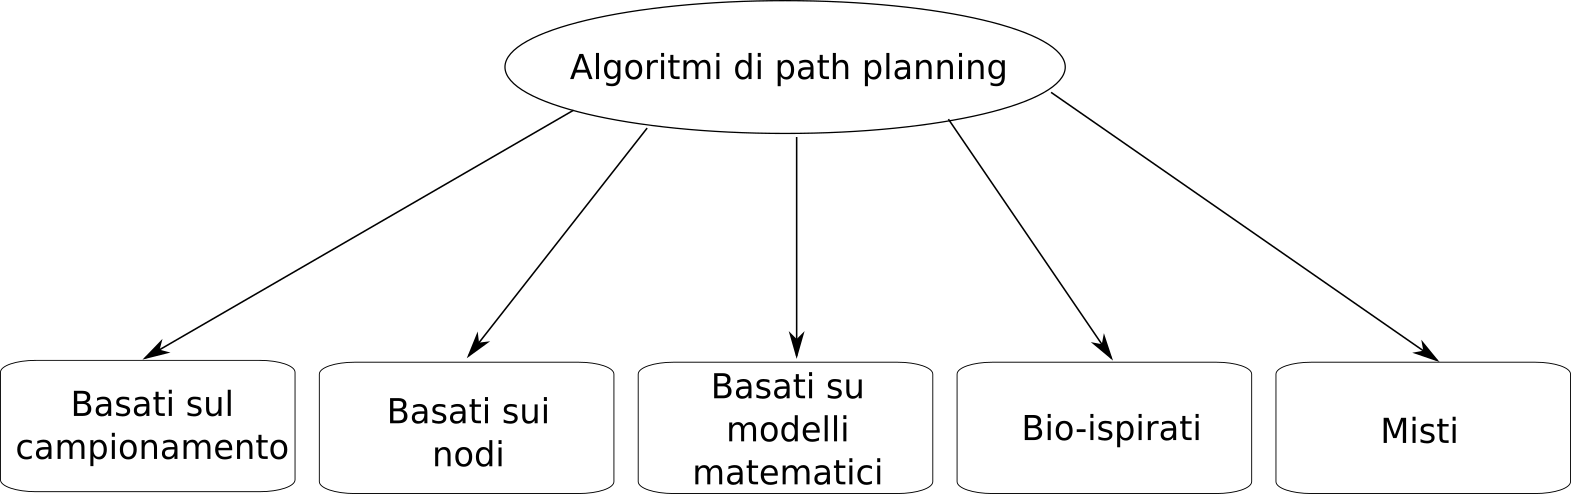
\includegraphics[width=0.7\textwidth]{SistemaQuadrirotore/Figure/Path}
	\caption{Classificazione dei tipi di algoritmi di Path Planning \cite{YangLiang2016SoR3}}
\end{figure}


\subsubsection{Algoritmi basati sul campionamento}

Gli algoritmi basati sul campionamento sono in grado di generare un percorso utile attraverso l'esplorazione casuale dell'ambiente. Fanno uso di concetti come nodi, celle o altre forme per determinare se il punto esplorato è compatibile con la soluzione da ricercare. Per effettuare la ricerca questo tipo di algoritmo necessitano di avere una conoscenza a priori dell'ambiente nella quale viene effettuata la ricerca.
Si possono suddividere le possibili implementazioni in due categorie:
\begin{itemize}
	\item \textbf{Attivi : } La soluzione avviene attraverso un esplorazione totalmente casuale di nuovi punti nella mappa in un solo passaggio si cerca di ottimizzarla
	\item \textbf{Passivi : }  La soluzione avviene attraverso la ricerca da un set di possibili soluzioni già determinate in un passaggio preliminare e attraverso un algoritmo di ricerca la migliore viene selezionata
\end{itemize}

%Questi algoritmi richiedono la conoscenza a priori di informazioni sull'ambiente e una rappresentazione matematica di questo. Si prevede di dividere l'ambiente in nodi o celle o altre forme. Avviene poi una ricerca attraverso una ricerca casuale. Questa categoria si può suddividere a sua volta in altre 2 categorie : attive e passive. Attive  si intende algoritmi che esploraro rapidamente in modo casuale per trovare il percorso migliore. Passivi algoritmi che si occupano di cercare la soluzione da percorsi già presenti come su di una mappa.



Nella categoria di algoritmi attivi ricade la Rapidly Exploring Random Tree (RRT). In questo algoritmo vengono generati nodi casualmente nello spazio con l'obbiettivo di raggiungere il punto obbiettivo dopo un numero non definito a priori di interazioni, \cite{Lavalle98rapidly-exploringrandom}. L'algoritmo ha il problema quindi di essere molto lento se l'ambiente è disordinato.

Per migliorare la velocità di convergenza ad una soluzione il precedente approccio viene arricchito nell'implementazione del Dinamic Domain RRT (DDRRT). In questo algoritmo attraverso l'introduzione di sfere attorno al nodo generato in ogni passaggio, si permette di determinare lo stato di esplorazione evitando di generare nodi in luoghi già esplorati, velocizzando il processo e superando in parte la limitazione della versione RRT, \cite{YangLiang2016SoR3}.

Generando una struttura dati ottimizzata per la ricerca utilizzando la Rapidly Exploring Random Graph (RRG), si può migliorare ulteriormente la l'approccio ottenuto attraverso RRT e DDRRT, velocizzando l'esplorazione. Il metodo prevede di generare ulteriori nodi intermedi, parallelizzando la generazione di percorsi alternativi attraverso il riempimento di un grafo di supporto, \cite{doi:10.1080/01691864.2013.805472}.

Esiste in bibliografia anche una versione ottimizzata della RRT, denominata RRT-Star (RRT*), \cite{ChoudhurySanjiban2013RSar}. Una versione in cui vengono eliminati i percorsi che si sono ottenuti e che probabilmente non sono ottimali, raffinando invece le connessioni, che vengono valutati dall'algoritmo  come migliori, di fatto una versione ad albero della RRG, \cite{YangLiang2016SoR3}. In questo modo si ottiene una soluzione ottimizzata rispetto agli altri algoritmi precedenti al prezzo però di non poter generare più percorsi contemporaneamente, utili per applicazioni con più robot, come mostrato nel lavoro \cite{doi:10.1080/01691864.2013.805472}. Questo approccio ha inoltre lo svantaggio di avere un costo computazione maggiore.

L'algoritmo Probabilistic Road Map (PRM) a differenza del RRT, prevede di generare più percorsi tra i vari nodi generati e valutarne successivamente la probabilità dell'efficacia di un percorso rispetto ad un altro. Attraverso un algoritmo di ricerca si testa la soluzione per discriminare la migliore, \cite{KavrakiL1994Prfp}.

Un approccio passivo è quello che viene definito Voronoi. Attraverso l'uso dei digrammi di Voronoi si determinano i nodi e le connessioni per generare il percorso. Il vantaggio è che in questo approccio si basa sulla minima distanza tra i nodi e con gli ostacoli. Si continua a suddividere l'ambiente fino a quando si ottiene collegamento tra tutti i segmenti che vengono man mano a formarsi, \cite{LuchnikovVA1999Vaov}. In questo approccio non è generare contemporaneamente il migliore percorso. Per sopperire a questa limitazione è necessario utilizzare in supporto un algoritmo di ricerca per discriminare il percorso migliore.

Tra i metodi attivi è presente anche l'algoritmo basato su energia potenziale. In questo algoritmo viene considerata una funzione potenziale attraverso interazione tra spazio percorribile e spazio occupato. Attraverso la generazione di una funzione potenziale funzione dell'ambiente e di pseudo forze si definisce il percorso da seguire. \'E molto facile da implementare e ha un costo computazionale basso, ha però il problema di presentare minimi locali e punti di ristagno , limitazione però facilmente superabile, \cite{RimonE1992Ernu}.

Riassumendo questi approcci si basano sull'esplorazione delle possibili soluzioni e la successiva valutazione per migliorare la forma ottenuta, sia in un solo passaggio che in più passaggi. L'algoritmo si applica in modo indipendente all'ambiente specifico, se non per la descrizione degli ostacoli e vincoli, aspetto concettualmente separato avendo la capacità di determinare le collisioni in modo autonomo, 
\cite{YangLiang2016SoR3}.


\subsubsection{Algoritmi basati sui nodi}
Questi algoritmi sono basati sull'utilizzo di nodi appartenenti ad un grafo scomposto, ricercando in mappe già pronte.

Tra questi algoritmi si trova l'algoritmo di Dijkstra, \cite{DIJKSTRA1959}. Conoscendo già un grafo in cui gli archi e i nodi sono stati pesati, si attua una ricerca per ridurre la funzione di costo. Partendo quindi dai nodi si genera il grafo con i pesi e poi si applica l'algoritmo. 

Un evoluzione di questo algoritmo è A-Star (A*), \cite{HartPeter1968AFBf}. Introducendo una stima euristica del costo durante il processo di ricerca si ottiene una più veloce velocità di convergenza. Per applicazioni con ostacoli dinamici si utilizza una versione modificata denominata D-Star (D*) che prevede di modificare i pesi nel grafo in funzione della configurazione degli ostacoli. 

Questo tipo di approccio però è limitativo in termini di soluzioni a causa della chiara incompletezza della struttura di configurazioni nell'ambiente. Di fatto si parla solamente di un algoritmo di ricerca non è in grado di generare un percorso ma solo una configurazione di sotto-percorsi già precostituiti, \cite{StentzA1994Oaep}, \cite{YangLiang2016SoR3}.

\subsubsection{Algoritmi basati su modelli matematici}
Questi metodi modellano l'ambiente  e il sistema modellando la funzione di costo con i limiti e vincoli per ottenere la soluzione ottimale. Equazioni e disequazioni vengono utilizzate per ottenere la soluzione migliore.
Vengono descritte matematicamente i vincoli cinematici e dinamici attraverso combinazioni di forme polinomiali, \cite{YangLiang2016SoR3}. 
Una categoria di approccio è quella attraverso algoritmi lineari. Si definisce una funzione di costo che contiene all'interno tutti i vincoli in termini di ottimizzazione della soluzione e le limitazioni del controllo, Eq. (\ref{eq:SistemaQuadrirotore_matmodel}).

\begin{equation}\label{eq:SistemaQuadrirotore_matmodel}
	J = f(u,x,y,z) + \varphi(x,y,z) + R(x,y,z)
\end{equation}
Dove $f(u,x,y,z)$ rappresenta il costo dell'attuazione, $\varphi(x,y,z)$ tiene conto dei vincoli geometrici e $R(x,y,z)$ una funzione che rappresenta la raggiungibilità di una posizione in modo da ottenere una convergenza più rapida, \cite{YangLiang2016SoR3}.
Attraverso questa formulazione si descrive completamente l'ambiente rendendo possibile anche tenere conto delle incertezze e fattori di disturbo.

Un altro tipo di algoritmo matematico è il Controllo Ottimo. Si imposta il problema da un punto di vista ottimo per il controllo utilizzando equazioni differenziali, \cite{AndersonS.J2009Auat}. Si utilizza una formulazione Hamiltoniana, con $H = \lambda^T(t) f\left[x(t),u(t)\right]$ per risolvere il problema, utilizzando una funzione di costo nella forma (\ref{eq:SistemaQuadrirotore_HamiltonCost}).

\begin{equation}\label{eq:SistemaQuadrirotore_HamiltonCost}
	J = \phi \left[x(t),u(t) \right] + \int_{t_0}^{t_f} \lambda^T(t) \{f\left[x(t),u(t)\right]-\dot{x}\} 
\end{equation}

In questa equazione $f\left[x(t),u(t)\right]$ rappresenta la dinamica del sistema.
Questi approcci descrivono completamente lo stato e le variabili in gioco. Risultano però essere complessa la risoluzione analitica. In bibliografia esistono strumenti che risolvono questo problema di ottimizzazione attraverso la sua discretizzazione, \cite{TricaudChristophe2010Aamf}.

\subsubsection{Algoritmi "bio-ispirati"}
Questi algoritmi mimano la natura per trovare una soluzione al problema. L'approccio è stocastico superando la soluzione basata su modelli matematici quando questi sono eccessivamente complessi.
Si può fare una suddivisione in due sottocategorie: Algoritmi evolutivi e reti neurali.

Gli algoritmi evolutivi cercano di imitare comportamenti e approcci presenti in natura. Grazie all'uso dell'algoritmo genetico si determina attraverso simulazioni la soluzione migliore. In \cite{6564703} viene mostrato una possibile sequenza genetica da utilizzare per sintetizzare  la soluzione. L'applicazione dell'algoritmo comporta di effettuare delle mutazioni di questa configurazione e di confrontarle tra di loro per mezzo di una funzione di fitness, in questo caso la minima distanza percorsa. Il processo prosegue iterativamente scartando le soluzioni peggiori. Raggiunta la condizione soddisfacente in almeno una soluzione, questa viene selezionata.
Altro esempio in bibliografia lo si trova in \cite{DuanHaibin2010Tppf}. In questo studio viene utilizzato un algoritmo che prende ispirazione dal rilascio di feromoni da parte delle formiche per determinare il percorso più breve, denominato Ant Colony Optimization (ACO) .

Le reti neurali esattamente come descritto precedentemente sono formati da modelli matematici che imitano il funzionamento dei neuroni in layer. In questa applicazione specifica si fa riferimento ad una formulazione dinamica che tiene conto dell'attività del neurone, Eq. (\ref{eq:SistemaQuadrirotore_DNN}).
\begin{equation}\label{eq:SistemaQuadrirotore_DNN}
	\dot{x}_i = -A x_i + (B -x_i) \left([I_i]^+ \sum_{j=1}^{k}w_{ij}[x_j]^+ \right) - (D + x_i) [I_i]^-
\end{equation}
Dove $x$ rappresenta l'attività del neurone, i parametri $A$, $B$ e $C$ sono collegati al rateo di decadimento del neuronee e $I$ gli input del neurone.
Le configurazioni posso essere molto varie. Per esempio in \cite{KassimA.A1992Anna}, viene descritta l'implementazione di una rete neurale, denominata Wave Expansion Neural Network (WENN), specifica per la'implementazione della pianificazione del percorso attraverso l'uso di campi potenziali. 


\subsubsection{Algoritmi misti}
Normalmente gli algoritmi presentati tendono a fondersi assieme per sopperire alle proprie limitazioni e trovare assieme una soluzione ottimale, con l'interviene un altro algoritmo che supporta il primo. Si può fare una suddivisione in due categorie: Embedded Multifusional Algorithms (EMA) e Ranked Multifusion Algorithm (RMA).
\begin{itemize}
	\item \textbf{EMA:} Gli algoritmi che vengono utilizzati lavorano contemporaneamente-
	\item \textbf{RMA:} La soluzione è ottenuta grazie alla partecipazione a livelli separati degli algoritmi scelti
\end{itemize}
Un esempio di EMA lo si trova applicato in \cite{SaberAhmedYousuf2008Sucb}: viene utilizzato l'algoritmo ACO nella quale localmente avviene una ottimizzazione utilizzando l'algoritmo A*.
In \cite{FeiYanYi-ShaLiuJi-ZhongXiao2013PPiC}, invece si implementa un approccio RMA: prima viene utilizzato l'algoritmo PRM e poi viene effettuata la ricerca attraverso l'uso di A* per trovare il percorso migliore.


\subsection{Pianificazione della traiettoria}
Pianificare la traiettoria significa generare il segnale di riferimento da dare al controllore per seguire il percorso trovato dall'algoritmo di generazione del cammino, in modo che questo si a eseguito correttamente. Per poter svolgere bene il suo compito bisogna tenere conto delle limitazioni cinematiche e dinamiche. La generazione di questi segnali avviene in genere attraverso l'interpolazione di funzioni conosciute. Queste funzioni poi inserite all'interno della valutazione devono essere compatibili con il sistema e le richieste della pianificazione.
Importante aspetto è la continuità, per limitare i disturbi e l'affaticamento degli attuatori. Traiettorie troppo discontinue son quindi da evitare anche in termini di capacità di seguire il percorso prestabilito, \cite{PathPlannigOverview}.

Una possibile impostazione del problema può essere quella di minimizzare il tempo di percorrenza. Si esprime la dinamica seguendo le coordinate curvilinee lungo il percorso geometrico e si analizzano le pseudo-velocità e le pseudo-accelerazioni lungo questo sistema di riferimento. Applicando le limitazione del caso su questi parametri, si trova la soluzione in termine di tempo necessario al percorrimento, \cite{PathPlannigOverview}. 
In \cite{BobrowJ.E2016TCoR} e \cite{HowieChoset2005PoRM}, viene descritto in dettaglio il metodo per minimizzare il tempo di percorrenza passante per un numero prestabilito di way-point, determinando le leggi orarie da imporre per l'inseguimento della traiettoria rispettando i vincoli imposti. 

Esiste un altro approccio a questo tipo di ottimizzazione che consiste nel valutare la soluzione suddividendo in porzioni il percorso e adottando in ogni sua parte, traiettorie programmate a priori. Per ogni sezione, in modo sequenziale, si eseguono traiettorie raccordate tra di esse, che seguono la sequenza di way-point prestabiliti ricercando contemporaneamente di soddisfare la minimizzazione del tempo di percorrenza globale, \cite{HowieChoset2005PoRM}. 

Un approccio utilizzato in robotica per velocizzare l'esecuzione del comando è minimizzare il tempo di esecuzione attraverso la generazione di profili di velocità trapezoidali. In questo caso non si tiene conto dell'azionamento degli attuatori e vengono prodotte traiettorie discontinue in termine di accelerazione. In \cite{DesTestCarm}, viene usato questo algoritmo per generare i segnali necessari al test MIL del controllore.
Per migliorare la risposta, si possono utilizzare funzioni spline, permettendo continuità in accelerazione e velocità, \cite{baseTesi}.
Attraverso l'uso delle spline, è possibile l'approccio per mezzo dell'uso di algoritmi genetici con lo scopo di ricercare una soluzione ottima, \cite{PathPlannigOverview}.

Nella ricerca di una traiettoria occorre anche minimizzare l'energia, valore stimato dalla coppia applicata dagli attuatori, direttamente collegata con il consumo di batteria, \cite{PathPlannigOverview}. Questo tipo di ottimizzazione permette inoltre una riduzione anche dello stress agli attuatori. Un esempio classico prevede l'uso delle B-spline, \cite{MartinBryanJ1999MMfO}. Nella soluzione a questo problema vengono in letteratura utilizzati anche spline cubiche \cite{Shin1986ADP}.
	
	%\chapter{Descrizione Autopilota}
	\chapter{Descrizione Autopilota}


\section{Descrizione del drone}


\todo[inline]{Descrizione del drone e dell'hardware dell'autopilota}
	\section{Descrizione del firmware PX4 Autopilot}
Il firmware utilizzato nelle simulazioni di software in the loop e processor in the loop è il PX4 Autopilot \cite{px4Firmware}, \cite{px4Guide}.
	
Questo software mette a disposizione diverse funzionalità per avere un sistema di gestione e controllo robusto e affidabile, implementato in diversi tipi di sistemi. L'implementazione non è quindi specifica solo a mezzi aerei di qualsiasi configurazione, ma anche a velicoli di terra, marini e razzi. Il software è open-source e vanta del contributo di parecchi sviluppatori, dagli esperti del settore a contributi di livello accademico. Lo sviluppo open-source permette quindi di aggiungere o modificare le funzionalità messe a disposizione in modo da soddisfare le proprie esigenze e arricchire il progetto generico di nuove funzionalità utili ad altri. Il sistema operativo sulla quale viene eseguito materialmente il codice può essere Nuttx o Linux/MacOS la cui distinzione principale in questa applicazione è solo nella gestione di task e thread.

Il sistema operativo Nuttx è un sistema RTOS (Real-Time Operating System) è svilupato appositamente per implementazioni embedeed. Essendo sviluppato per un contesto specifico ha tutte le caratteristiche necessarie per essere eseguito in sistemi che devono avere prestazioni migliori con poche risorse disponibili. Vengono utilizzati gli standard POSIX e ANSI \cite{Nuttx}. Inoltre, sono implementate funzionalità di programmazione concorrenziale per l'esecuzione di processi in parallelo. Le funzionalità del firmware vengono eseguite in questo sistema come task separati e ogni task può eseguire diversi thread.
Nell'implementazione su sistemi Linux/MacOS invece i moduli sono eseguiti come thread del processo principale, non c'è quindi una distinzione tra threads e tasks, oltre a non essere ottimizzato per sistemi embedeed.


\subsection{Architettura del software}
Il firmware è principalmente suddiviso in due categorie di moduli:
\begin{itemize}
	\item \textbf{Flight stack} : composta dalla parte che stima lo stato del sistema e il relativo controllo
	\item \textbf{Middleware} : composta dalle interfacce che collegano i vari moduli interni di PX4 tra di loro e verso l'esterno, con la possibilità di integrare gli hardware utilizzati.
\end{itemize}

Il sistema quindi separa le varie funzionalità in moduli separati, eseguiti in modo indipendente che scambiano i dati e comandi tra di loro e con l'esterno attraverso messaggi asincroni.
Nella figura \ref{fig:px4.architettura} è riportato lo schema di alto livello del software di PX4 e la sua modularità.

\begin{figure}
	\centering
	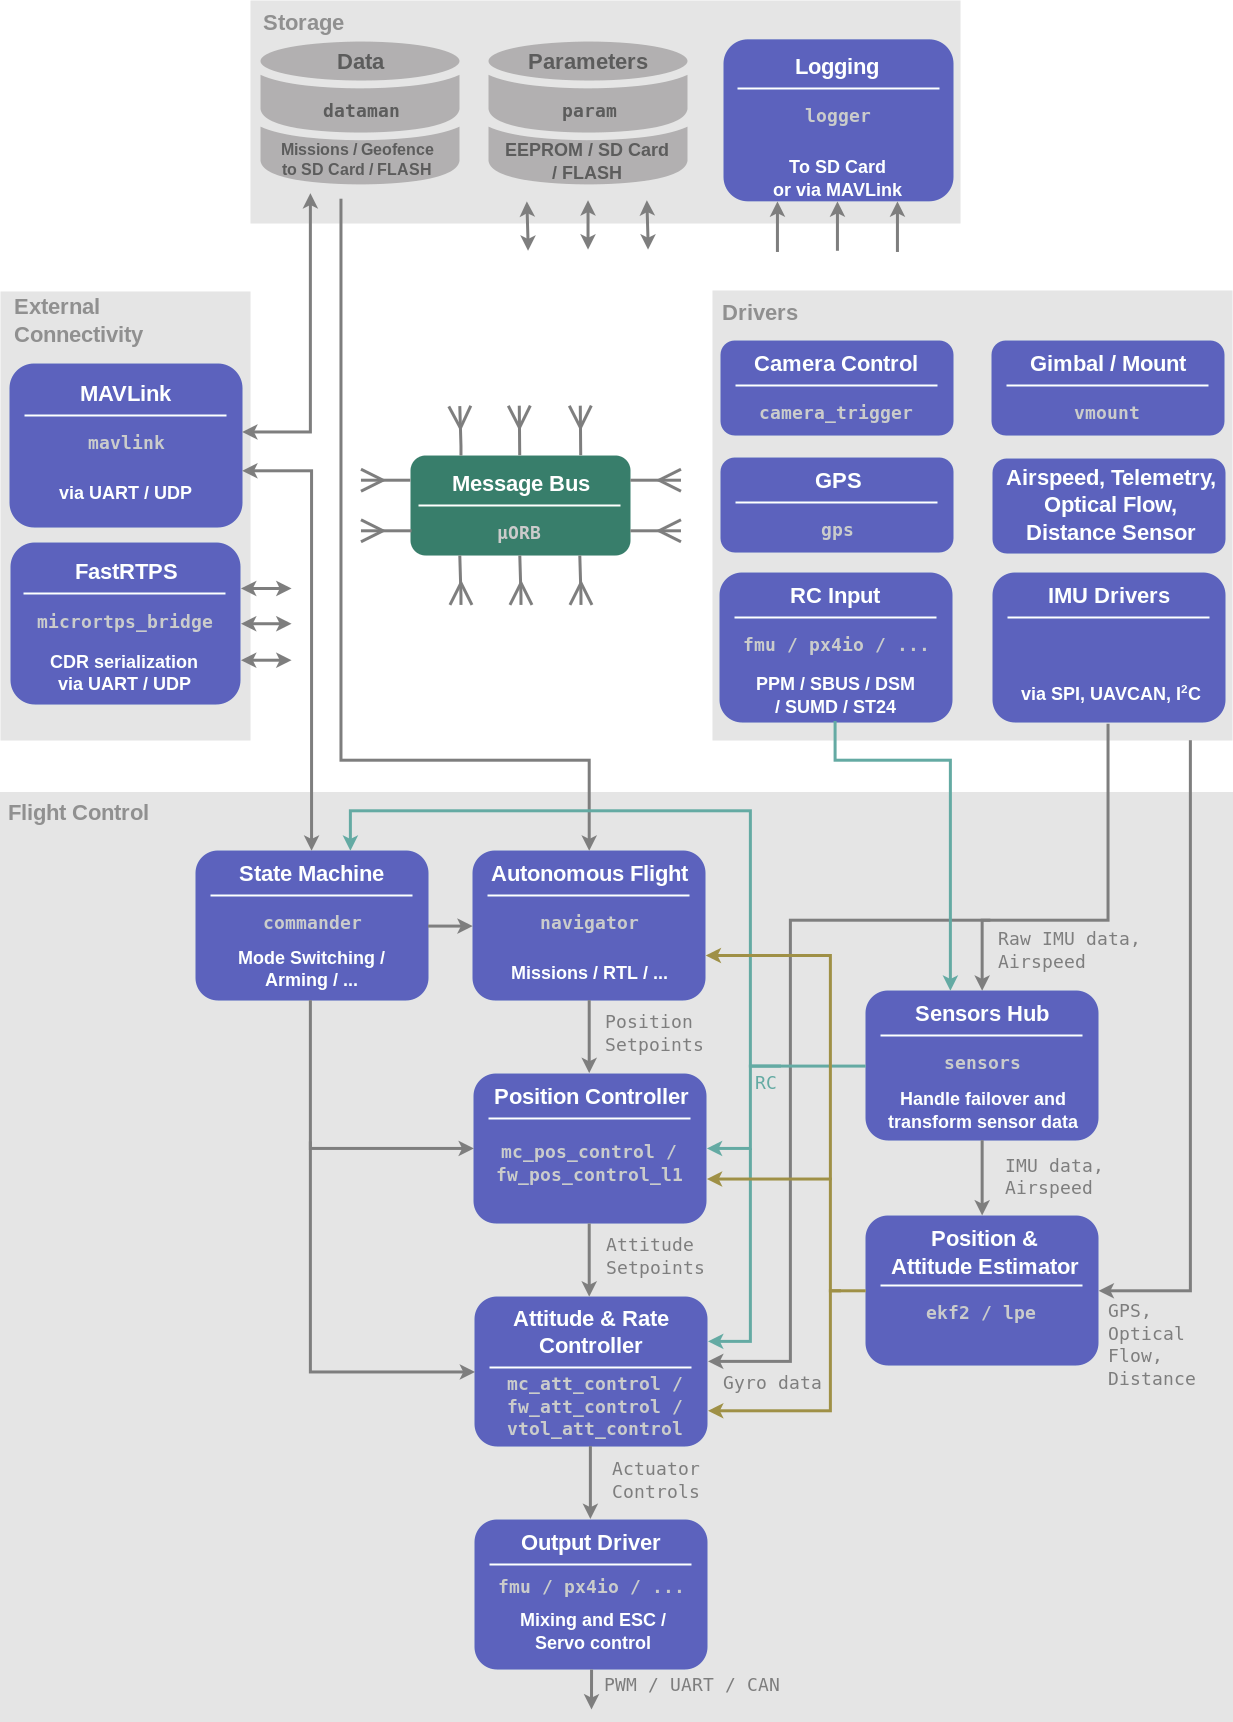
\includegraphics[width=0.8\textwidth]{DescrizioneAutopilota/Figure/PX4_Architecture}
	\caption{Architettura del codice di PX4 Autopilot, \cite{px4Guide}}
	\label{fig:px4.architettura}
\end{figure}
\subsubsection{Flight stack}
Il flight stack, mostrato in figura \ref{fig:px4.flightstack} è l'insieme di moduli che si occupano della stima dello stato del sistema e di tutti le funzionalità per il controllo,la guida e la navigazione. Esiste anche un modulo per interfacciarsi con il volo manuale attraverso radiocomando.
	\begin{figure}[ht]
	\centering
	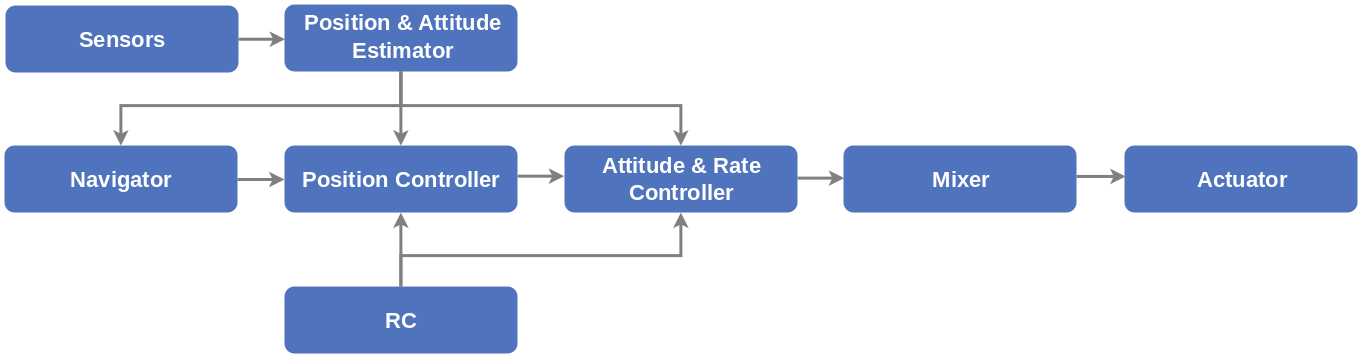
\includegraphics[width=1\textwidth]{DescrizioneAutopilota/Figure/PX4_High-Level_Flight-Stack}
	\caption{Architettura del flight stack di PX4, \cite{px4Guide}}
	\label{fig:px4.flightstack}
\end{figure}
\paragraph{Estimator}
L'estimator è il modulo che prendendo i dati da uno o più sensori determina lo stato attuale del velivolo. E' possibile selezionare diversi tipi di estimato, quello selezionato in questo caso è uno stimatore con filtro di Kalman.
\paragraph{Controller}
Si occupa di prendere in input i vari punti della pianificazione e confrontarli con lo stato attuale determinato dell'estimator. In questo modo vengono determinati i segnali di comando di output che saranno poi elaborati dal mixer. Questa funzionalità è implementata da più moduli, suddividendo la dinamica lenta e la dinamica veloce del drone. Verrà disabilitata la sua funzionalità per sostituirla con l'applicazione sviluppata su Simulink.
\paragraph{Mixer}
Il mixer si occupa di tradurre i segnali del comandi normalizzati di rollio, imbardata, beccheggio e manetta, da consegnare all'hardware che genera gli impulsi pwm utilizzati per il controllo del motore.
\subsubsection{Middleware}
Questo insieme di moduli si occupa invece di tutte le comunicazioni interne tra processi e tra PX4 e il mondo esterno. \'E composta principalmente dai driver per i sensori, i canali di comunicazione verso l'esterno e il bus di trasmissione di messaggi attraverso $\micro$ORB e MAVLink, \cite{MAVLink}. In questo contesto ricade anche  la connessione con un simulatore per testare il codice generato nelle varie fasi di validazione.
\subsection{Strumenti per lo sviluppo del codice}
Il sistema operativo utilizzato per lo sviluppo è Ubuntu 18.04.5 LTS, nella quale è stato installato MATLAB 2020a. Viene inoltre installato il tool "Embeded Coder Support Package for PX4 Autopilots", seguendo la guida, \cite{PX4MATLAB}. La versione di Ubuntu  installata però non è pienamente compatibile in quanto non è presente di default il software necessario al lancio delle simulazioni da parte di Simulink, ovvero "xterm", che va installato manualmente. La versione di PX4 utilizzata è quella prevista dalla guida \cite{PX4MATLAB}, ovvero la versione "1.8.0". Risulta inoltre necessario installare anche la versione di Java 8 e ROS-Melodic contenente il software Gazebo.

L'intero codice del firmware PX4 viene messo a disposizione attraverso la piattaforma github, \cite{PX4-FIRMWAREGIT}. Il progetto contiene all'interno le toolchain necessarie per compilare il sistema nei vari sistemi operativi. Agendo sulle varie possibili configurazioni di compilazione è possibile modificare e aggiunge delle funzionalità. Modificando le impostazioni di compilazione si può generare il programma finale da caricare ed eseguire sull'autopilota.
Sono presenti anche delle configurazioni per effettuare l'analisi e la verifica del codice generato attraverso l'utilizzo di un ambiente simulato. I simulatori che presentano una configurazione di base sono : Gazebo, jMAVSim , AirSim, Xplane. Per quanto riguarda questa tesi, verrà utilizzato il software Gazebo sfruttando parzialmente il codice già presente e adottando alcune modifiche. Nulla vieta comunque di poter collegare un simulatore diverso attraverso la creazione di un interfaccia dati con il firmware. Infatti, la connessione viene effettuata attraverso UDP o seriale, utilizzando su essa il protocollo MAVLink.

Per la generazione del codice sorgente da implementare nel firmware PX4, si fa utilizzo delle funzionalità aggiunte a MATLAB/Simulink dal tool "Embeded Coder Support Package for PX4 Autopilots", \cite{PX4MATLAB}. Dopo l'installazione di questo pacchetto vengono aggiunti alla libreria standard di Simulink, alcuni blocchetti utili all'interfacciamento con le restanti parti del firmware di PX4. Attraverso l'utilizzo di messaggi $\micro$ORB avvengono infatti le comunicazioni con i moduli eseguiti parallelamente alla configurazione del firmware: stimatore, sensori, attuatori ecc.

Nella creazione del modello in Simulink, si è tenuto conto del fatto che i dati necessari al controllo, venissero prelevati dallo stimatore di default di PX4, a differenza del lavoro svolto precedentemente in \cite{DesTestCarm}, nella quale si sono implementati le funzioni dei sensori e uno stimatore specifico.

Attraverso l'uso dei messaggi passati dal Firmware a Simulink quindi si sono implementati i controllori come spiegato in dettaglio nel capilo precedente. Nella Figura (\ref{fig:in}), viene mostrato l'implementazione su simulink necessaria a leggere lo stato del drone.

\begin{figure}
	\centering
	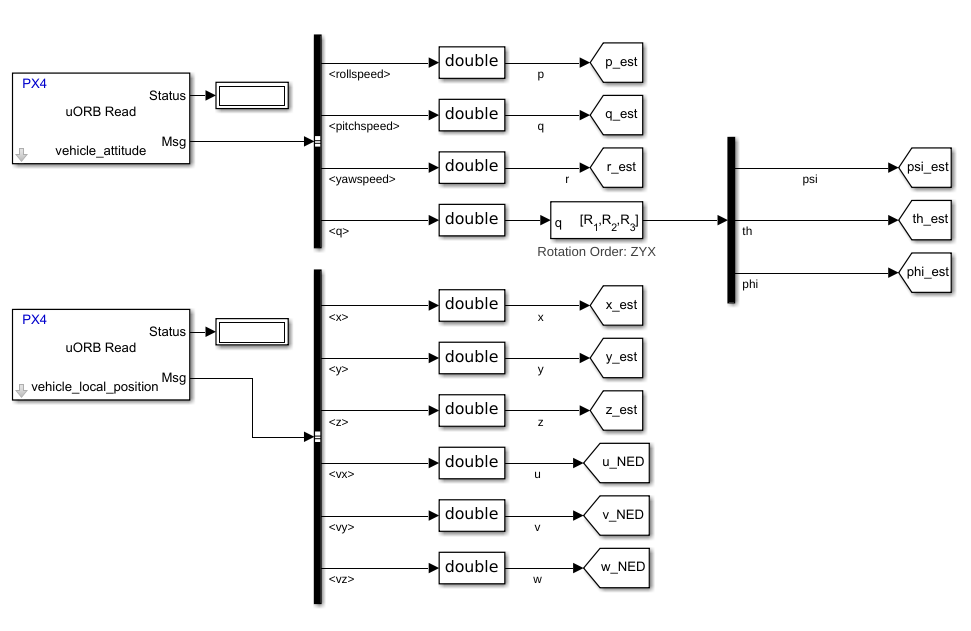
\includegraphics[width=0.6\textwidth]{DescrizioneAutopilota/Figure/IN}
	\caption{Interfaccia di input del modulo di controllo implementato su Simulink}
	\label{fig:in}
\end{figure}

Analogamente avviene il collegamento in output del sistema di controllo con l'apposito modulo della libreria, Figura (\ref{fig:out}).

\begin{figure}
	\centering
	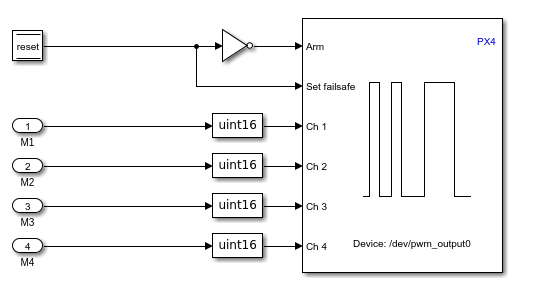
\includegraphics[width=0.5\textwidth]{DescrizioneAutopilota/Figure/OUT}
	\caption{Interfaccia di output del modulo di controllo implementato su Simulink}
	\label{fig:out}
\end{figure}

Utilizzando quindi questi moduli in input e output, il Coder è in grado generare il codice sorgente, incapsularlo in un modulo di PX4 e compilarlo. Da questo si ottiene quindi un file eseguibile con il sistema PX4 compilato e integrato in esso il controllo implementato. 

Nativamente il tool di Simulink sopracitato non permette l'utilizzo dell'ambiente Gazebo, ma solamente il simulatore jMavSim. Per questo è stato studiato il processo di lancio della simulazione integrato nel tool e la documentazione sui collegamenti tra il firmware PX4 e Gazebo nelle simulazioni SIL effettuate senza utilizzare Simulink. Attraverso la scrittura di uno script, presente in appendice, si è superata questa limitazione, rendendo possibile l'utilizzo di Gazebo per effettuare le simulazioni SIL. In Figura (\ref{fig:ig:INTERSIL}), viene mostrata la configurazione utilizzata per effettuare le simulazioni SIL. Come è possibile osservare nel caso si compili il codice per effettuare SIL, viene compilato all'interno del firmware un modulo che ha lo scopo specifico di interfacciare il simulatore con il Firmware. Il controllore utilizzato è integrato come modulo all'interno del firmware stesso.

\begin{figure}[!h]
	\centering
	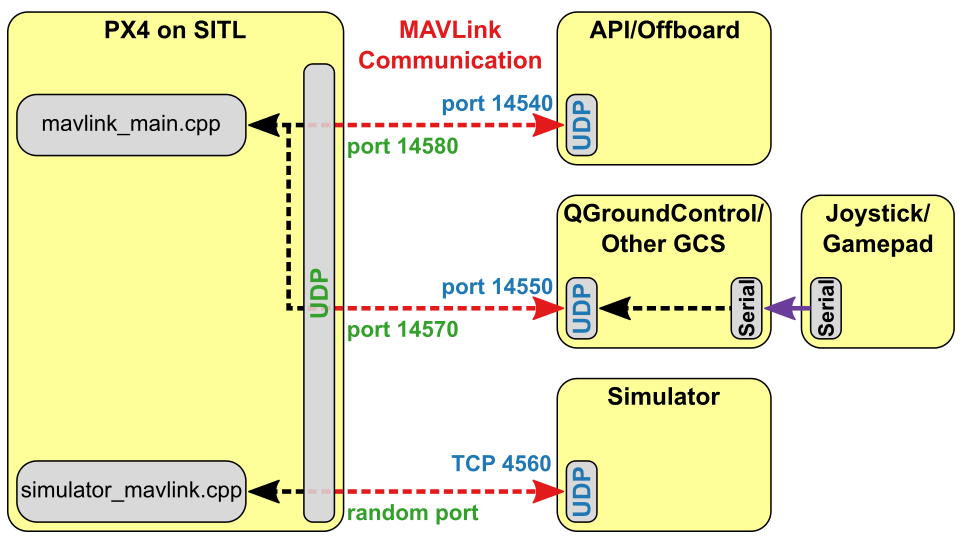
\includegraphics[width=0.5\textwidth]{DescrizioneAutopilota/Figure/INTERSIL}
	\caption{Configurazione per effettuare le simulazioni SIL}
	\label{fig:ig:INTERSIL}
\end{figure}



	\section{Gazebo}
\label{section:gazebo}

Il toolbox di simulazione utilizzato, come precedentemente accennato, è Gazebo. Questo software permette di utilizzare un motore fisico interno del simulatore, denominato Open Dynamic Engine (ODE), \cite{ODE}. ODE è un motore fisico che permette di risolvere in tempo reale la dinamica degli oggetti posizionati all'interno del mondo di simulazione, determinando contemporaneamente lo stato di collisione, mantenendo la compatibilità con eventuali librerie aggiunte ed eseguite in contemporanea. Gazebo infatti mette a disposizione la sua Aplication Programming Interface (API), necessaria alla scrittura di codice sorgente per aggiungere funzionalità particolari come ad esempio la generazione dei dati da parte dei sensori e l'applicazione di forze aerodinamiche sul corpo del quadricottero, \cite{Gazebo}. 

Gazebo permette anche di utilizzare l'insieme di framework di Robot Operating System 2 (ROS2), della quale lo stesso Gazebo fa parte, includendo quindi una vastità di funzionalità e prodotti già implementati per applicazioni di robotica, \cite{ROSGAZEBO}.

All'interno progetto di sviluppo del firmware di PX4, \cite{PX4FIRMWARE}, è presente un esempio di simulazione utilizzando Gazebo, con relativi codici sorgenti di plugin utili nella cartella "Tools/sitl\_gazebo". Nella simulazione di default sono già presenti le funzionalità dei sensori, IMU e GPS, e l'interfaccia di comunicazione utilizzante il protocollo MavLink attraverso la rete locale del computer Host, Figura (\ref{fig:ig:INTERSIL}).
Per effettuare le simulazioni SIL all'interno del progetto è stato aggiunto il modello tridimensionale del drone, Figura (\ref{fig:DRONECAD}). Modificando i file di configurazione di gazebo sono stati assegnati i valori di massa e inerzia coerentemente come in tabella (\ref{tab:DRONE}).
E stato inoltre modificato il file del codice sorgente relativo al modulo software "gazebo\_motor\_model.cpp", come è possibile visionare in appendice, per implementare nella simulazione le leggi polinomiali trovate sperimentalmente riguardante le forze e i momenti sui rotori, Figura (\ref{fig:pwmTM}), in modo da avere un confronto più preciso con le simulazione effettuate in MIL.

\begin{figure}
	\centering
	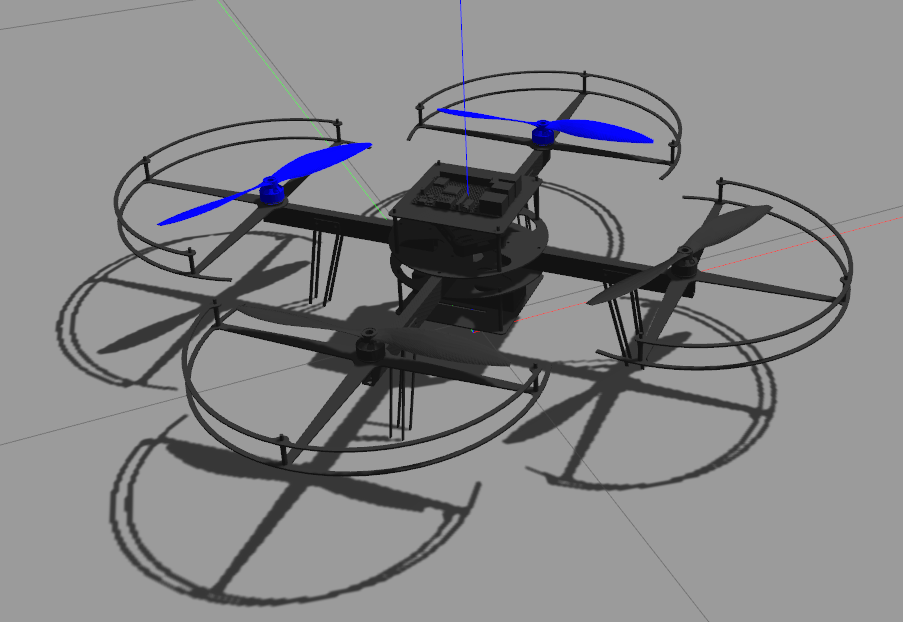
\includegraphics[width=0.4\textwidth]{DescrizioneAutopilota/Figure/DRONECAD}
	\caption{Drone utilizzato nella simulazione in Gazebo}
	\label{fig:DRONECAD}
\end{figure}

Il lancio della simulazione, avviene in contemporeanea al lancio del software di PX4 attraverso l'utilizzo di uno script., allegato in appendice. Questo script richiama il software con le corrette impostazioni ed avvia la simulazione collegando il simulatore al programma dell'autopilota.


	%\chapter{Simulazioni}
	\chapter{Simulazioni}
\label{cap:simulazioni}
In questo capitolo vengono presentate in dettaglio le simulazioni effettuate in SIL e MIL. Inoltre è presente una sezione in cui verrà riportata parzialmente la soluzione per le simulazioni in PIL. Nella sezione di MIL verrà descritto il modello dei sensori e dello stimatore usato nella precedente tesi, \cite{DesTestCarm}, per il confronto. Diverse osservazioni e confronti verranno fatti tra le simulazioni. La parte finale descriverà la conclusione del lavoro e eventuali sviluppi futuri.

Nelle simulazioni verranno utilizzati i seguenti percorsi:
\begin{itemize}
		\item \textbf{STEP: } Questa sequenza di waypoint definisce una fase di decollo stazionando a 3 m dal suolo, Tabella (\ref{tab:STEP})
		\item \textbf{SQUARE: } Sequenza di decollo seguita da un percorso a 2.5 m di altezza di forma quadrata con lato di 3 m e atterraggio nell'ultima posizione, Tabella (\ref{tab:SQUARE})
		\item \textbf{BUTTERFLY: } Sequenza di decollo seguita da un percorso a croce su un area di 3 m per lato, Tabella (\ref{tab:BUTTERFLY})
		\item \textbf{SNAKE: } Sequenza di decollo fino a 2.5 m, seguita da un percorso di forma varia descritta nella Tabella (\ref{tab:SNAKE})
\end{itemize}

\section{Simulazione SIL}

\begin{figure}
	\centering
	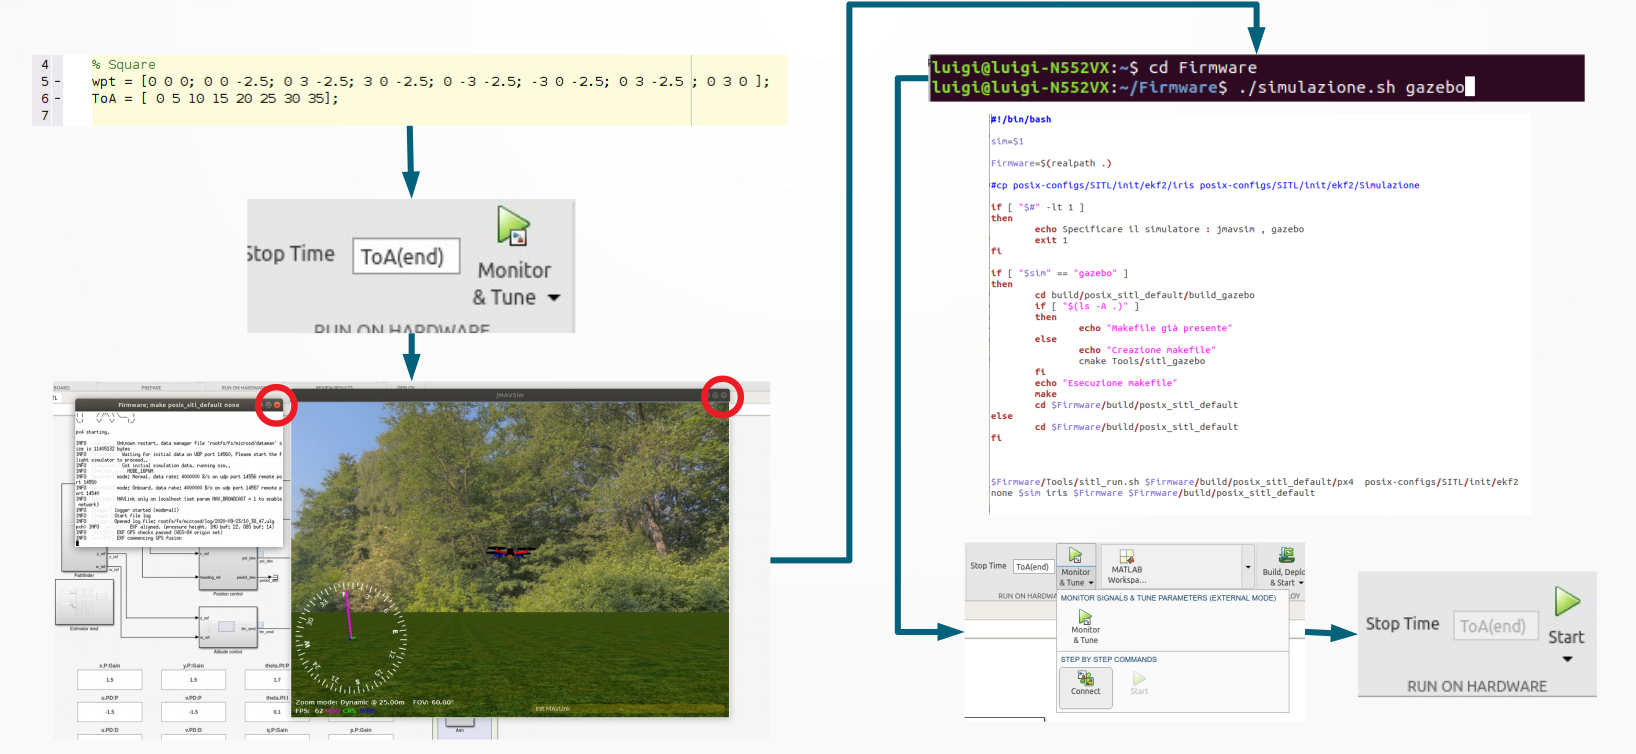
\includegraphics[width=1\textwidth]{DescrizioneAutopilota/Figure/SIMSIL}
	\caption{Descrizione del procedimento per effettuare la simulazione SIL}
	\label{fig:SIMSIL}
\end{figure}

Per effettuare la simulazione è necessaria la generazione del codice, processo che avviene in modo automatico utilizzando Simulink. Dopo aver selezionato nell'apposito file di inizializzazione la sequenza di waypoint necessari per la generazione della traiettoria, si lancia una prima fase di simulazione standard, come riportato nella guida, \cite{px4Guide}. Si termina il software lanciato dal tool, jMavSim, e attraverso la linea di comando si esegue lo script scritto appositamente per questo scopo, allegato in appendice.
Una volta avviata la simulazione e gazebo pronto, è possibile premendo il tasto "Connect", connettere i parametri presenti su Simulink con il codige generato nel software e gli strumenti necessari all'acquisizione dei dati di simulazione, e avviare il modulo di controllo. Nella Figura (\ref{fig:SIMSIL}), è riportato una descrizione grafica di questo procedimento.


\begin{table}
	\centering
	\begin{tabular}{c c c c}
		\hline
		Tempo alla posizione [s] &  x [m] & y [m] & z [m]\\
		\hline
		0 & 0 & 0 & 0 \\
		3 & 0 & 0 & -3 \\
		5 & 0 & 0 & -3 \\
		\hline
	\end{tabular}	
	\caption{Descrizione del segnale STEP}
	\label{tab:STEP}
\end{table}

\begin{table}
	\centering
	\begin{tabular}{c c c c}
		\hline
		Tempo alla posizione [s] &  x [m] & y [m] & z [m]\\
		\hline
		0 & 0 & 0 & 0 \\
		5 & 0 & 0 & -2.5 \\
		10 & 0 & 3 & -2.5 \\
		15 & 3 & 0 & -2.5 \\
		20 & 0 & -3 & -2.5 \\
		25 & -3 & 0 & -2.5 \\
		30 & 0 & 3 & -2.5 \\
		35 & 0 & 3 & 0 \\
		\hline
	\end{tabular}	
	\caption{Descrizione del segnale SQUARE}
	\label{tab:SQUARE}
\end{table}

\begin{table}
	\centering
	\begin{tabular}{c c c c}
		\hline
		Tempo alla posizione [s] &  x [m] & y [m] & z [m]\\
		\hline
		0 & 0 & 0 & 0 \\
		5 & 0 & 0 & -2.5 \\
		10 & 3 & -3 & -2.5 \\
		15 & 3 & 3 & -2.5 \\
		20 & -3 & -3 & -2.5 \\
		25 & -3 & 3 & -2.5 \\
		30 & 3 & -3 & -2.5 \\
		\hline
	\end{tabular}	
	\caption{Descrizione del segnale BUTTERFLY}
	\label{tab:BUTTERFLY}
\end{table}

\begin{table}
	\centering
	\begin{tabular}{c c c c}
		\hline
		Tempo alla posizione [s] &  x [m] & y [m] & z [m]\\
		\hline
		0 & 0 & 0 & 0 \\
		5 & 0 & 0 & -2.5 \\
		10 & 3 & -3 & -2.5 \\
		15 & 3 & 0 & -2.5 \\
		25 & -3 & 0 & -2.5 \\
		30 & -3 & 3 & -2.5 \\
		40 & 3 & 3 & -2.5 \\
		45 &	3 & 6 & -2.5 \\
		55 & -3 & 6 & -2.5 \\
		70 & -3 & -3 & -2.5 \\
		80 & 3 & -3 & -2.5 \\
		90 & 3 & -3 & 0 \\
		\hline
	\end{tabular}	
	\caption{Descrizione del segnale SNAKE}
	\label{tab:SNAKE}
\end{table}

\clearpage
\subsection{PID}

Vengono qui riportate le simulazioni SIL utilizzando la configurazione denominata PID nel capitolo \ref{cap:controllore}.

\subsubsection{STEP}
\begin{figure}
	\centering
	\begin{subfigure}{0.45\textwidth}
		\centering
		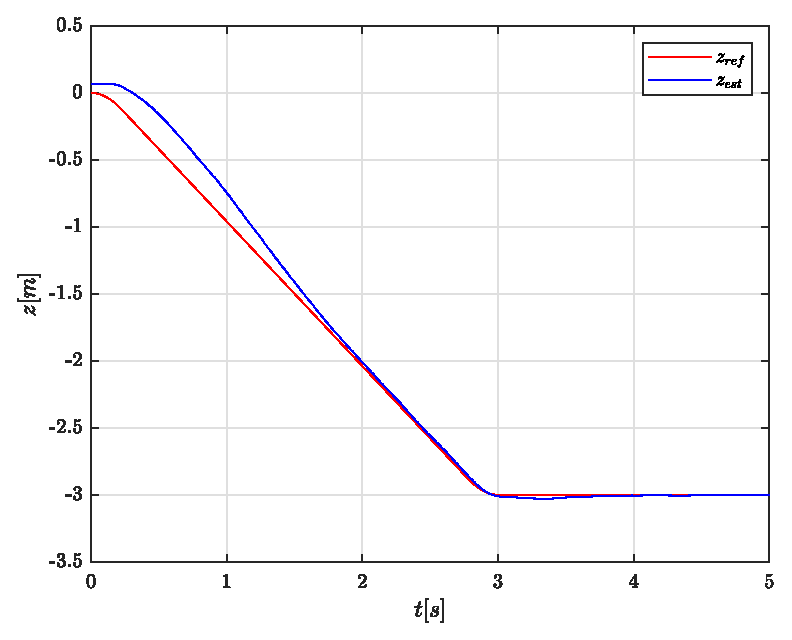
\includegraphics[width=1\textwidth]{Simulazioni/Figure/PID/STEP/AltitudeControlPos}
		\caption{Controllo posizione}
		\label{fig:STEPerrposzPID}
	\end{subfigure}
	\hfill
	\begin{subfigure}{0.45\textwidth}
		\centering
		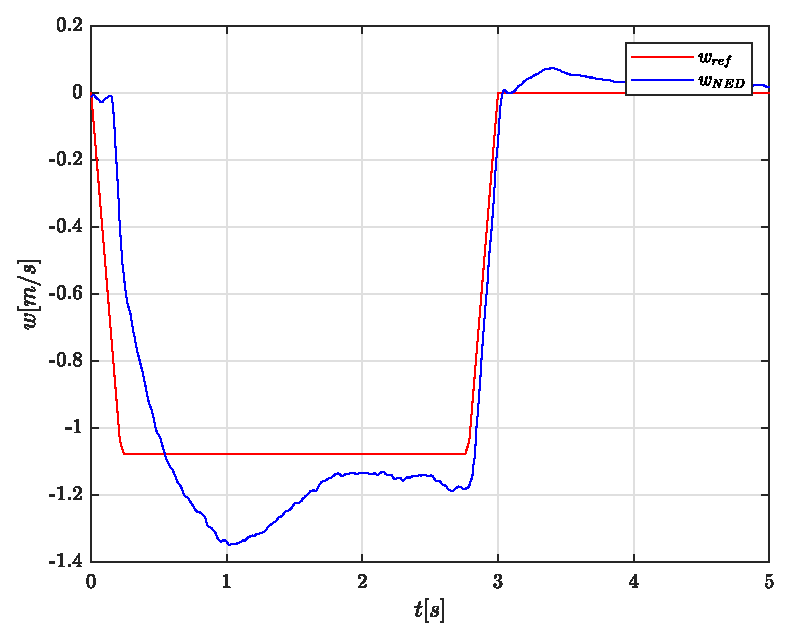
\includegraphics[width=1\textwidth]{Simulazioni/Figure/PID/STEP/AltitudeControlVel}
		\caption{Controllo velocità}
	\end{subfigure}
	\caption{Risposta del controllore PID di quota al segnale STEP}
	\label{fig:STEPerrvelzPID}
\end{figure}

\begin{figure}
	\centering
	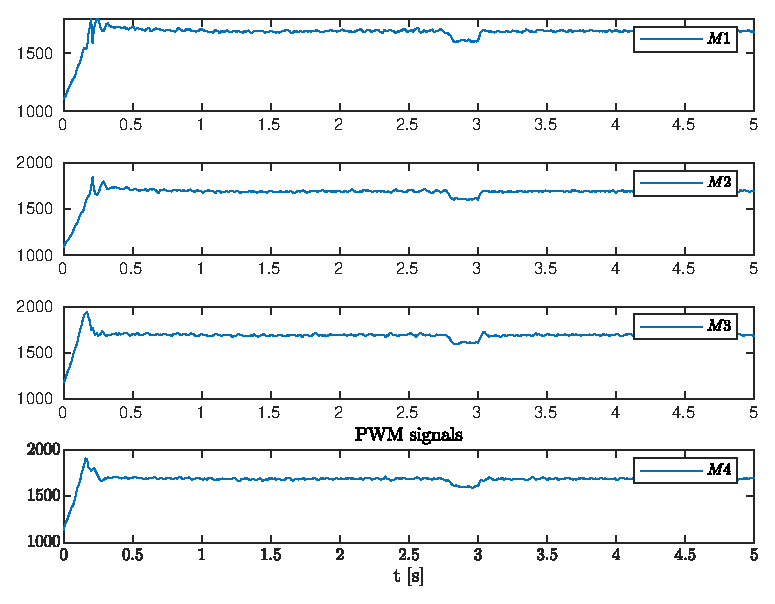
\includegraphics[width=0.5\textwidth]{Simulazioni/Figure/PID/STEP/PWM}
	\caption{Segnali PWM del controllore PID al segnale STEP}
	\label{fig:STEPerrPWMzPID}
\end{figure}

In questa simulazione si oserva come il controllore PID risponda correttamente al comando di decollo. L'errore iniziale risulta essere maggiore nella prima fase a causa dell'errore misurato inizialmente sulla quota. Nel proseguire della manovra il sistema riesce correttamente a minimizzare corettamente l'errore di posizione, Figura (\ref{fig:STEPerrposzPID}). L'inseguimento del rateo di salita risulta essere imprecisa nella fase iniziale, presentando un overshoot e un successivo assestamento lento è impreciso. Nella fase di livellamento però sia l'overshoot che l'errore stazionario si riduce, Figura (\ref{fig:STEPerrposzPID}). Il segnale PWM in uscita del controllore risulta essere abbastanza regolare, senza presentare oscillazioni eccessive, rimanendo in un range nominale e non presentando saturazione.

\subsubsection{SQUARE}

\begin{figure}
	\centering
	\begin{subfigure}{0.45\textwidth}
		\centering
		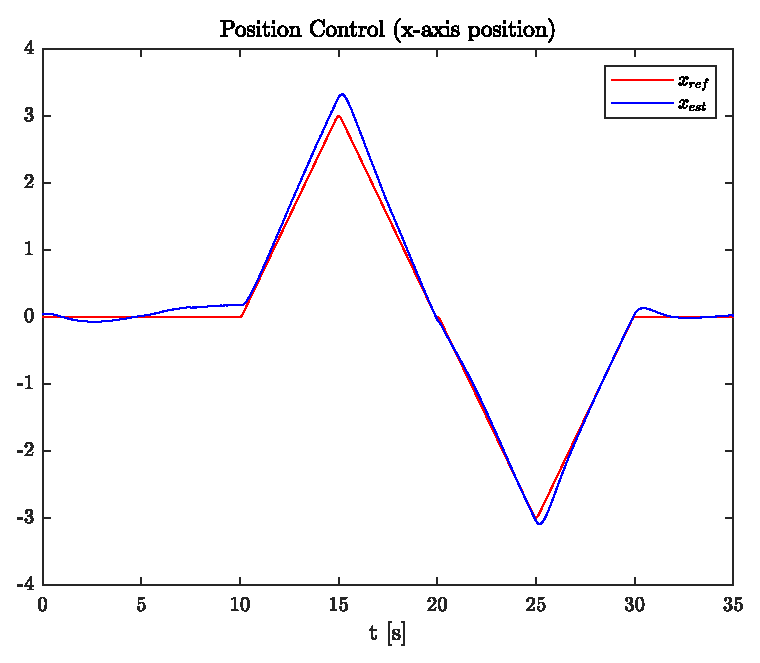
\includegraphics[width=1\textwidth]{Simulazioni/Figure/PID/SQUARE/PositionControlXPos}
		\caption{Controllo posizione lungo x}
		\label{fig:SQUAREerrposxPID}
	\end{subfigure}
	\hfill
	\begin{subfigure}{0.45\textwidth}
		\centering
		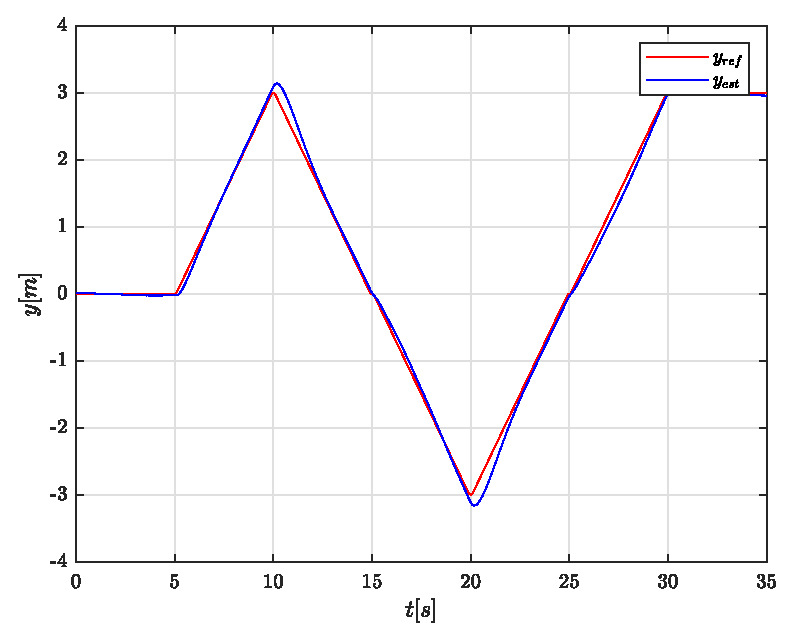
\includegraphics[width=1\textwidth]{Simulazioni/Figure/PID/SQUARE/PositionControlYPos}
		\caption{Controllo posizione lungo y}
		\label{fig:SQUAREerrposyPID}
	\end{subfigure}
	\\
	\begin{subfigure}{0.45\textwidth}
		\centering
		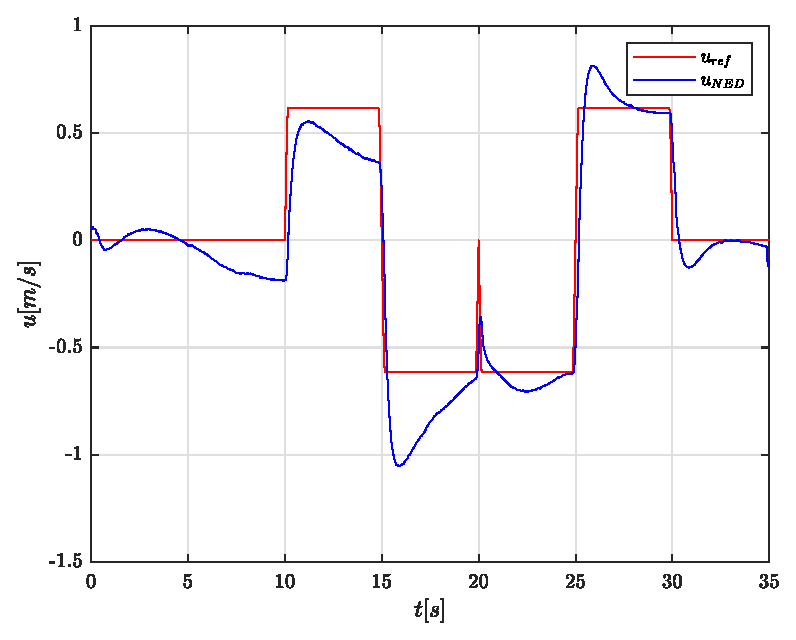
\includegraphics[width=1\textwidth]{Simulazioni/Figure/PID/SQUARE/PositionControlXVel}
		\caption{Controllo velocità lungo x}
		\label{fig:SQUAREerrvelxPID}
	\end{subfigure}
	\hfill
	\begin{subfigure}{0.45\textwidth}
		\centering
		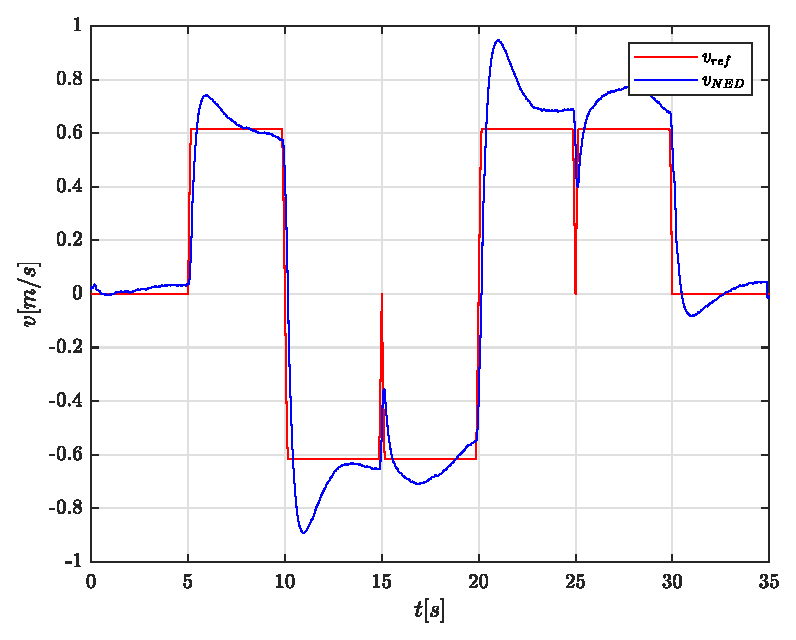
\includegraphics[width=1\textwidth]{Simulazioni/Figure/PID/SQUARE/PositionControlYVel}
		\caption{Controllo velocità lungo y}
		\label{fig:SQUAREerrvelyPID}
	\end{subfigure}
	\caption{Risposta in posizione con controllore interno PID al comando SQUARE}
\end{figure}

\begin{figure}
	\centering
	\begin{subfigure}{0.45\textwidth}
		\centering
		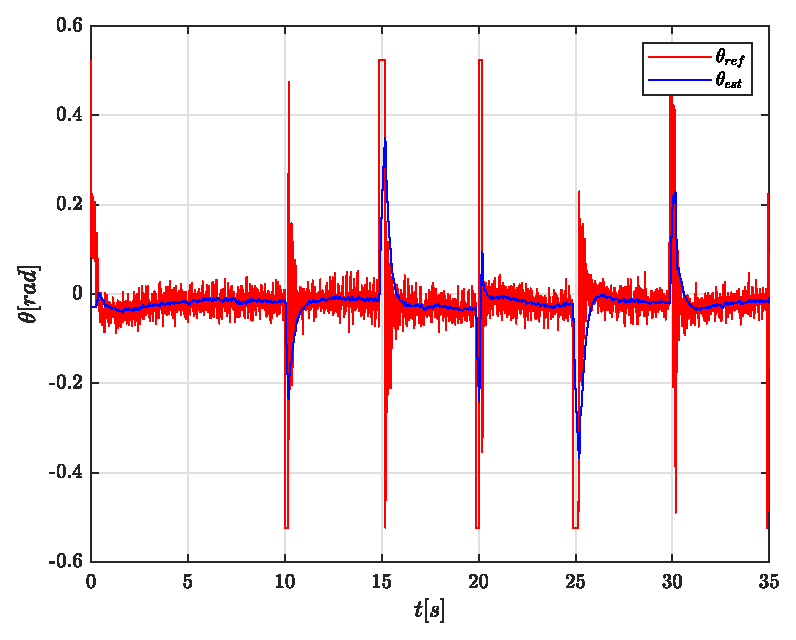
\includegraphics[width=1\textwidth]{Simulazioni/Figure/PID/SQUARE/AttitudeControlPitch}
		\caption{Controllo beccheggio}
		\label{fig:SQUAREerrbecPID}
	\end{subfigure}
	\hfill
	\begin{subfigure}{0.45\textwidth}
		\centering
		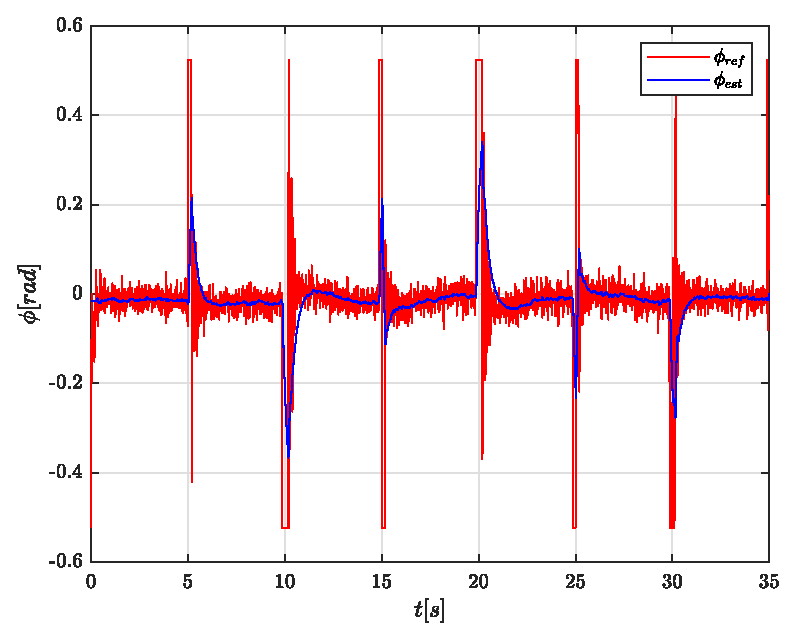
\includegraphics[width=1\textwidth]{Simulazioni/Figure/PID/SQUARE/AttitudeControlRoll}
		\caption{Controllo rollio}
		\label{fig:SQUAREerrrolPID}
	\end{subfigure}
	\hfill
	\begin{subfigure}{0.45\textwidth}
		\centering
		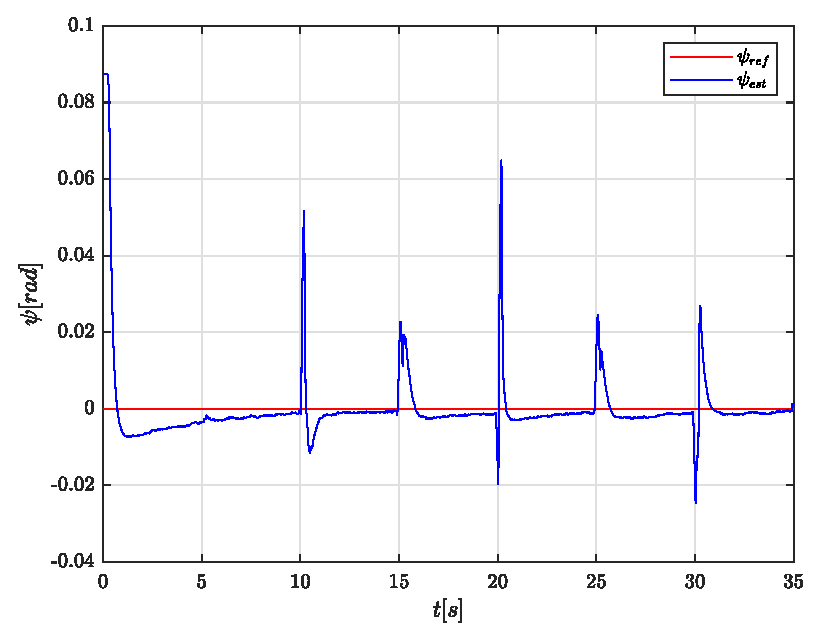
\includegraphics[width=1\textwidth]{Simulazioni/Figure/PID/SQUARE/AttitudeControlYaw}
		\caption{Controllo imbardata}
		\label{fig:SQUAREerryawPID}
	\end{subfigure}
	\caption{Risposta dell' assetto con controllore interno PID al comando SQUARE}
\end{figure}


\begin{figure}
	\centering
	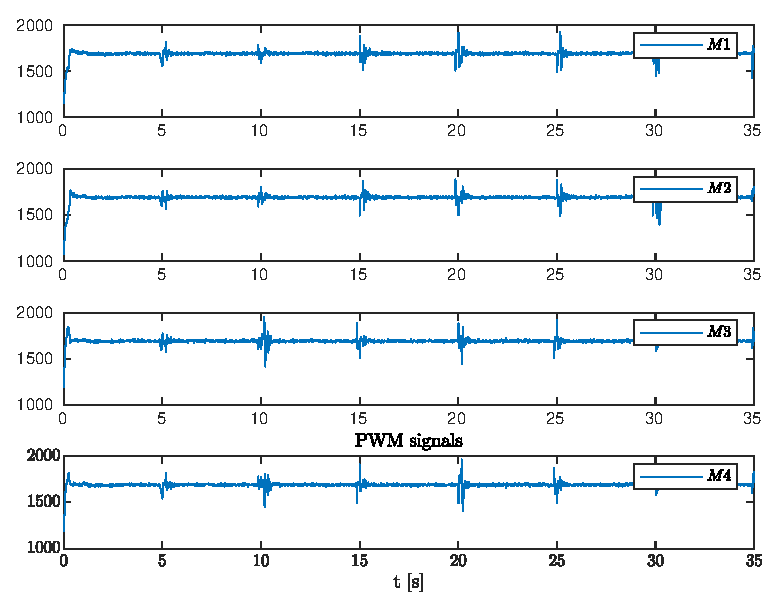
\includegraphics[width=0.5\textwidth]{Simulazioni/Figure/PID/SQUARE/PWM}
	\caption{Segnali PWM del controllore PID al segnale SQUARE}
	\label{fig:SQUAREPWMPID}
\end{figure}
\begin{figure}
	\centering
	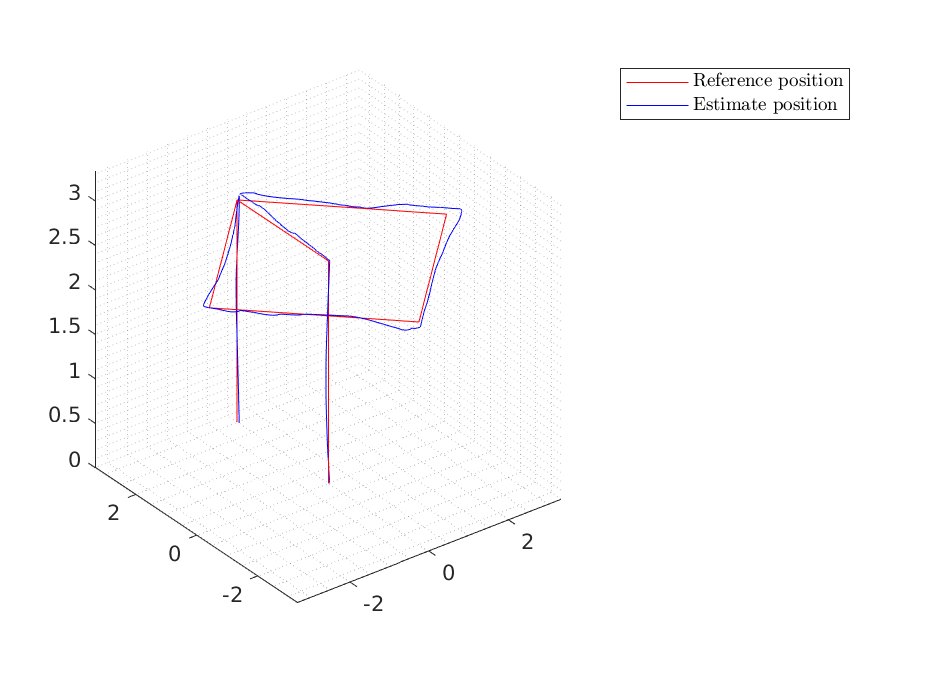
\includegraphics[width=1\textwidth]{Simulazioni/Figure/PID/SQUARE/Trajectory}
	\caption{Traiettoria percorsa con controllore PID al segnale SQUARE}
	\label{fig:SQUAREtraPID}
\end{figure}

In questa simulazione viene mostrata la capacità di muoversi nello spazio rispetto alle coordinate $x$ e $y$. L'errore di posizione osservato risulta essere relativamente piccolo. Gli incrementi di questo risultano essere maggiori nella fase di decollo iniziale e nell'attuazione dei cambi di velocità, Figure (\ref{fig:SQUAREerrposyPID}) e (\ref{fig:SQUAREerrposyPID}). L'inseguimento da parte del controllore PID nei confronti della velocità presenta alcuni picchi di overshoot quando questa subisce repentine variazioni, mostrando però l'assestamento successivo verso la riduzione asintotica della differenza. La risposta in velocità risulta essere molto rapida, Figure (\ref{fig:SQUAREerrvelyPID}) e (\ref{fig:SQUAREerrvelyPID}). Osservando i segnali di riferimento generati dal Position Control per l'Attitude Control,nelle Figure (\ref{fig:SQUAREerrbecPID}) e (\ref{fig:SQUAREerrrolPID}), si nota la presenza di intervalli in cui il controllore di posizione è in saturazione. Il segnale di riferimento generato dal Position Control presenta una componente di rumore. Il velivolo riesce comunque a seguire mediamente questo segnale, portandosi in condizione di assetto corretto per seguire la velocità di traslazione. Per quanto riguarda l'angolo di imbardata, con riferimento costante, presenta a causa degli effetti di accoppiamento tra le rotazioni lungo gli assi $x$ e $y$, degli scostamenti. Il sistema risponde molto bene per ridurre questo tipo di errore, come è osservabile nella Figura (\ref{fig:SQUAREerryawPID}). Anche in questa simulazione il segnale PWM generato è molto pulito e non presenta oscillazioni di ampiezza rilevante rispetto al valore medio, Figura (\ref{fig:SQUAREPWMPID}). Osservando la Figura (\ref{fig:SQUAREtraPID}), si osserva come il controllore sia in grado di percorrere la traiettoria prestabilita in modo efficacie, con alcune fasi di scostamento nelle variazione della direzione. La fase di atterraggio non presenta particolari criticità.

\subsubsection{BUTTERFLY}

\begin{figure}
	\centering
	\begin{subfigure}{0.45\textwidth}
		\centering
		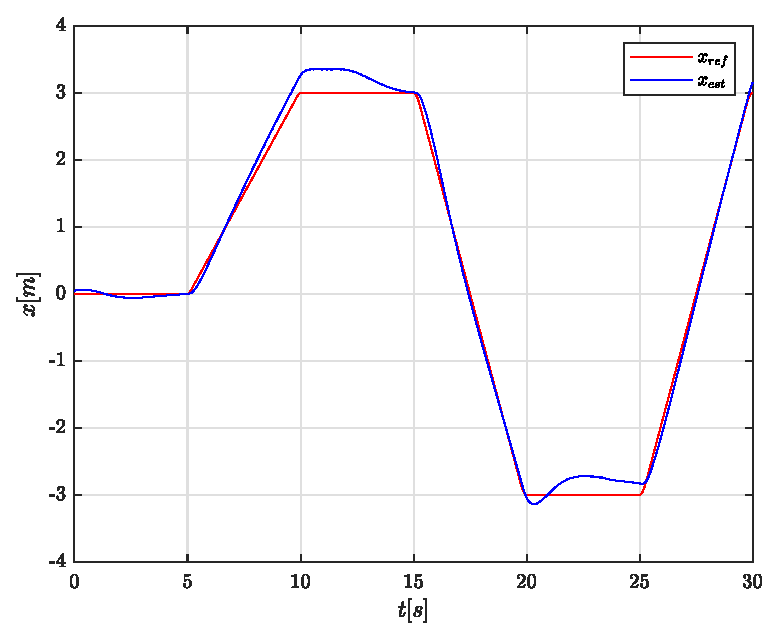
\includegraphics[width=1\textwidth]{Simulazioni/Figure/PID/BUTTERFLY/PositionControlXPos}
		\caption{Controllo posizione lungo x}
		\label{fig:BUTTERFLYerrposxPID}
	\end{subfigure}
	\hfill
	\begin{subfigure}{0.45\textwidth}
		\centering
		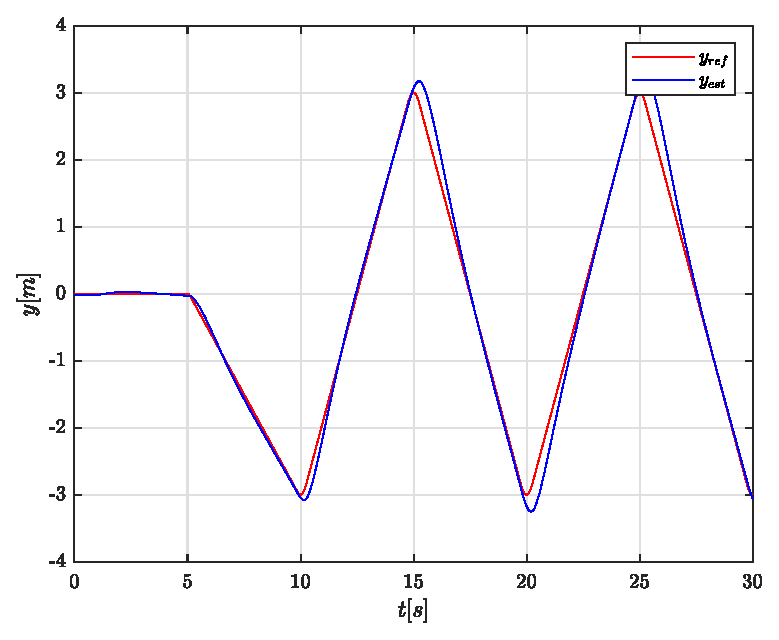
\includegraphics[width=1\textwidth]{Simulazioni/Figure/PID/BUTTERFLY/PositionControlYPos}
		\caption{Controllo posizione lungo y}
		\label{fig:BUTTERFLYerrposyPID}
	\end{subfigure}
	\\
	\begin{subfigure}{0.45\textwidth}
		\centering
		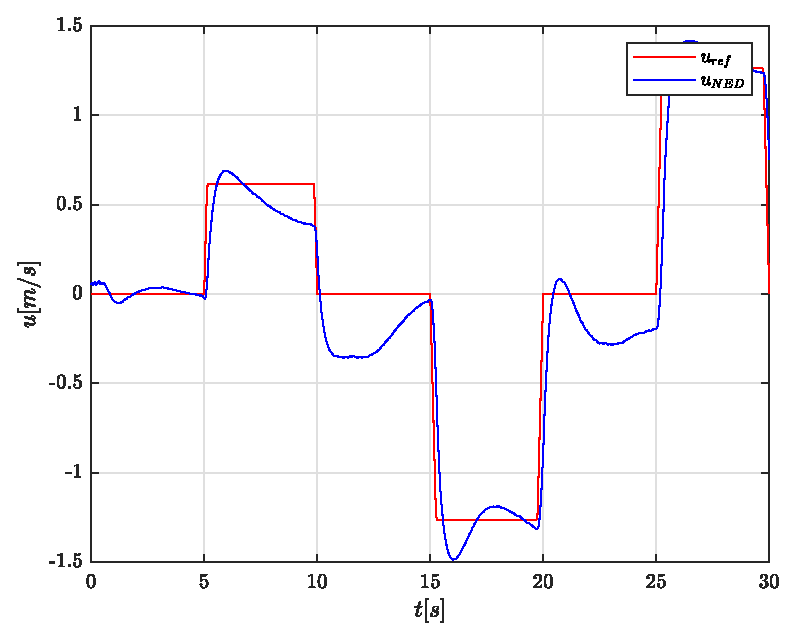
\includegraphics[width=1\textwidth]{Simulazioni/Figure/PID/BUTTERFLY/PositionControlXVel}
		\caption{Controllo velocità lungo x}
		\label{fig:BUTTERFLYerrvelxPID}
	\end{subfigure}
	\hfill
	\begin{subfigure}{0.45\textwidth}
		\centering
		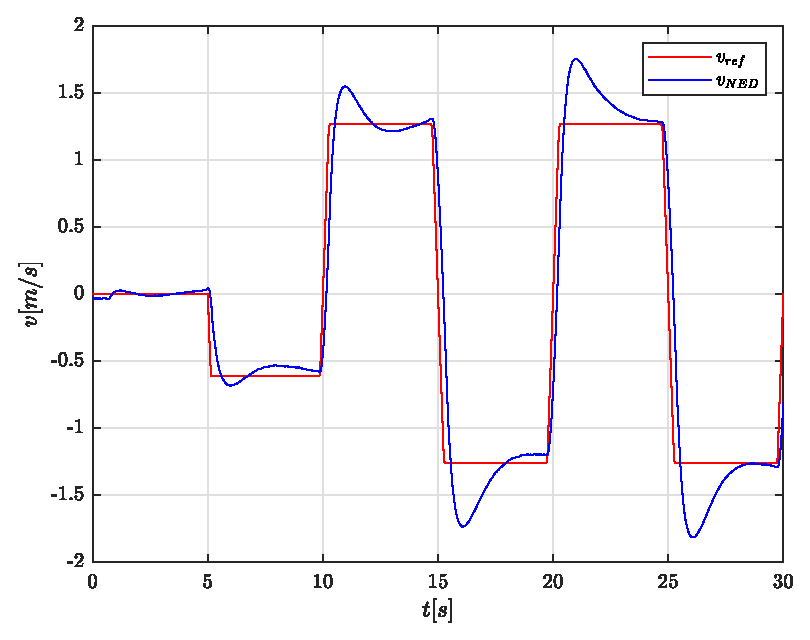
\includegraphics[width=1\textwidth]{Simulazioni/Figure/PID/BUTTERFLY/PositionControlYVel}
		\caption{Controllo velocità lungo y}
		\label{fig:BUTTERFLYerrvelyPID}
	\end{subfigure}
	\caption{Risposta in posizione con controllore interno PID al comando BUTTERFLY}
\end{figure}

\begin{figure}
	\centering
	\begin{subfigure}{0.45\textwidth}
		\centering
		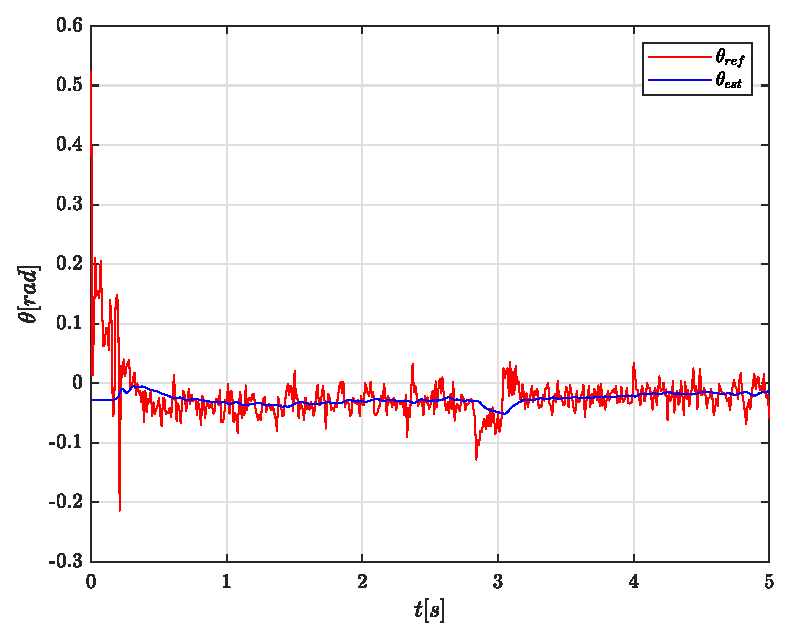
\includegraphics[width=1\textwidth]{Simulazioni/Figure/PID/BUTTERFLY/AttitudeControlPitch}
		\caption{Controllo beccheggio}
		\label{fig:BUTTERFLYerrbecPID}
	\end{subfigure}
	\hfill
	\begin{subfigure}{0.45\textwidth}
		\centering
		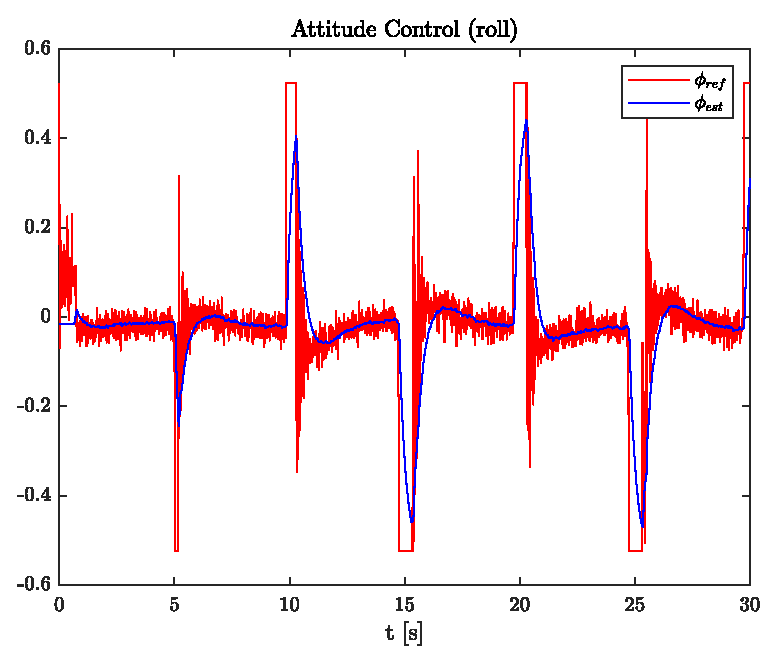
\includegraphics[width=1\textwidth]{Simulazioni/Figure/PID/BUTTERFLY/AttitudeControlRoll}
		\caption{Controllo rollio}
		\label{fig:BUTTERFLYerrrolPID}
	\end{subfigure}
	\hfill
	\begin{subfigure}{0.45\textwidth}
		\centering
		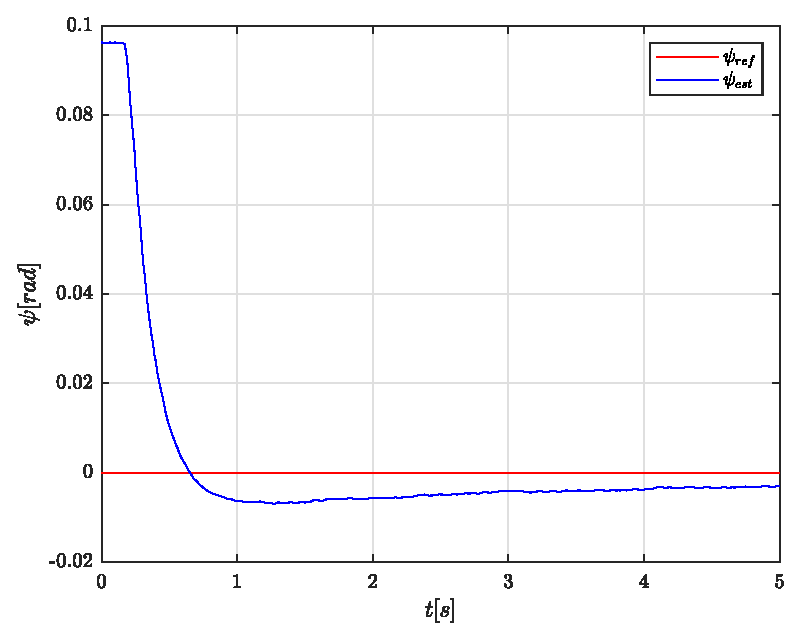
\includegraphics[width=1\textwidth]{Simulazioni/Figure/PID/BUTTERFLY/AttitudeControlYaw}
		\caption{Controllo imbardata}
		\label{fig:BUTTERFLYerryawPID}
	\end{subfigure}
	\caption{Risposta dell' assetto con controllore interno PID al comando BUTTERFLY}
\end{figure}


\begin{figure}
	\centering
	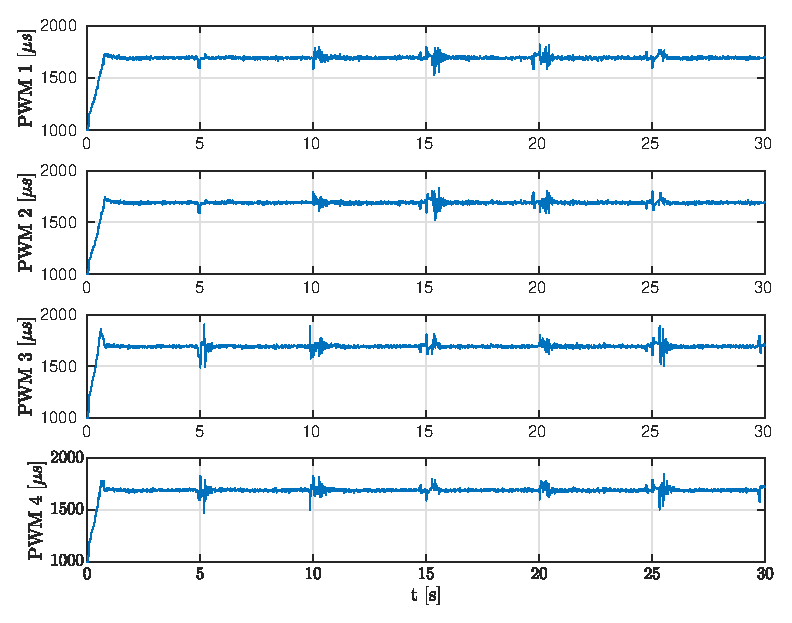
\includegraphics[width=0.5\textwidth]{Simulazioni/Figure/PID/BUTTERFLY/PWM}
	\caption{Segnali PWM del controllore PID al segnale BUTTERFLY}
	\label{fig:BUTTERFLYPWMPID}
\end{figure}
\begin{figure}
	\centering
	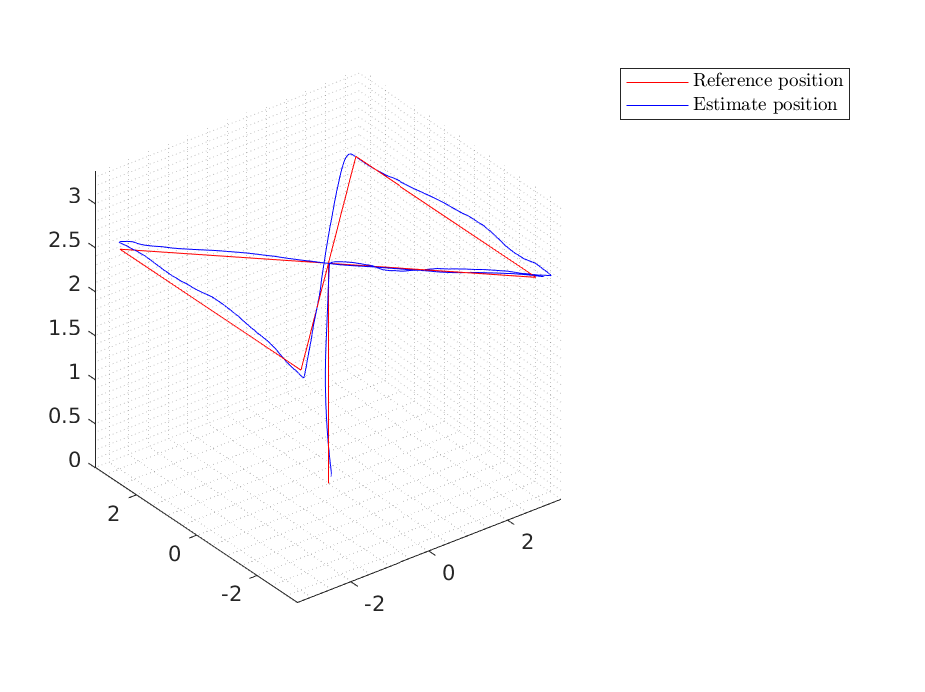
\includegraphics[width=1\textwidth]{Simulazioni/Figure/PID/BUTTERFLY/Trajectory}
	\caption{Traiettoria percorsa con controllore PID al segnale SQUARE}
	\label{fig:BUTTERFLYtraPID}
\end{figure}

In questa simulazione viene eseguito un percorso più lungo rispetto alla precedente in termine di spazio percorso, inoltre il cambiamento di direzione comandato al raggiungimento del waypoint è maggiore. La risposta è molto simile alla precedente. Anche in questa simulazione l'errore di posizione osservato risulta essere piccolo. Gli incrementi risultano maggiori nella fase di decollo iniziale e nell'attuazione dei cambi di velocità, Figure (\ref{fig:BUTTERFLYerrposyPID}) e (\ref{fig:BUTTERFLYerrposyPID}). Sono presenti i picchi di overshoot nella risposta in velocità, con una fase successiva di assestamento. La risposta in velocità è rapida, Figure (\ref{fig:BUTTERFLYerrvelyPID}) e (\ref{fig:BUTTERFLYerrvelyPID}). Nelle Figure (\ref{fig:BUTTERFLYerrbecPID}) e (\ref{fig:BUTTERFLYerrrolPID}), si nota la presenza di intervalli in cui il controllore di posizione è in saturazione e la presenza di un oscillazione rispetto ad un valore medio. Il segnale PWM generato è molto pulito e non presenta oscillazioni di ampiezza rilevante rispetto al valore medio, Figura (\ref{fig:BUTTERFLYPWMPID}). Come osservabile in Figura (\ref{fig:BUTTERFLYtraPID}), il controllore è in grado di percorrere efficacemente la traiettoria prestabilita con alcuni scostamenti in presenza di cambiamenti repentini di direzione.

\subsubsection{SNAKE}

\begin{figure}
	\centering
	\begin{subfigure}{0.45\textwidth}
		\centering
		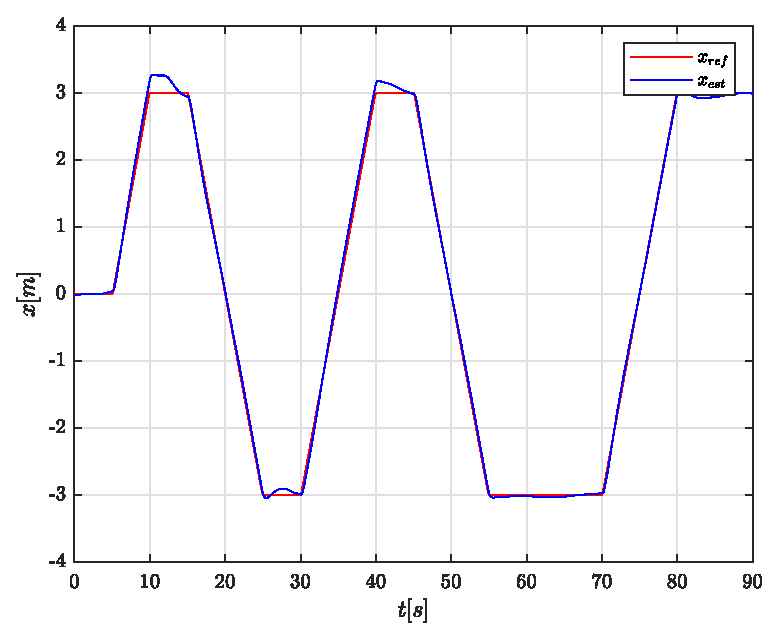
\includegraphics[width=1\textwidth]{Simulazioni/Figure/PID/SNAKE/PositionControlXPos}
		\caption{Controllo posizione lungo x}
		\label{fig:SNAKEerrposxPID}
	\end{subfigure}
	\hfill
	\begin{subfigure}{0.45\textwidth}
		\centering
		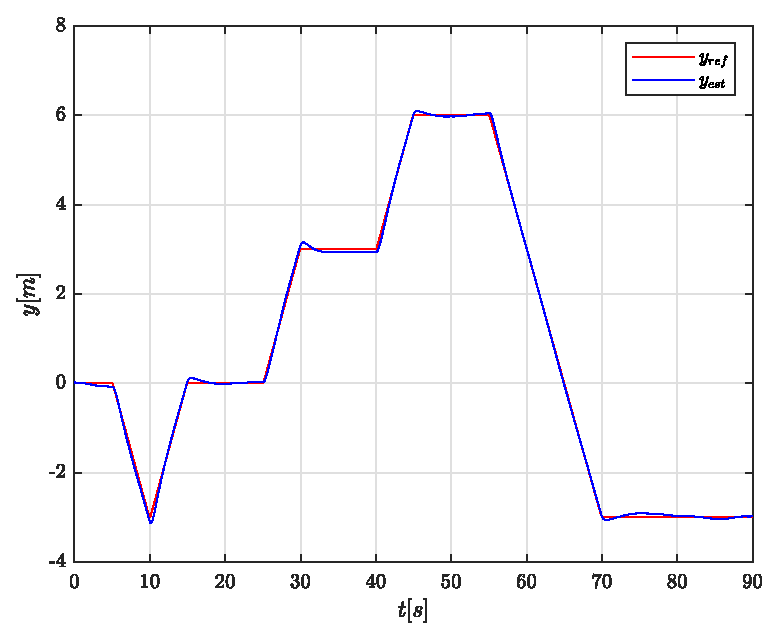
\includegraphics[width=1\textwidth]{Simulazioni/Figure/PID/SNAKE/PositionControlYPos}
		\caption{Controllo posizione lungo y}
		\label{fig:SNAKEerrposyPID}
	\end{subfigure}
	\\
	\begin{subfigure}{0.45\textwidth}
		\centering
		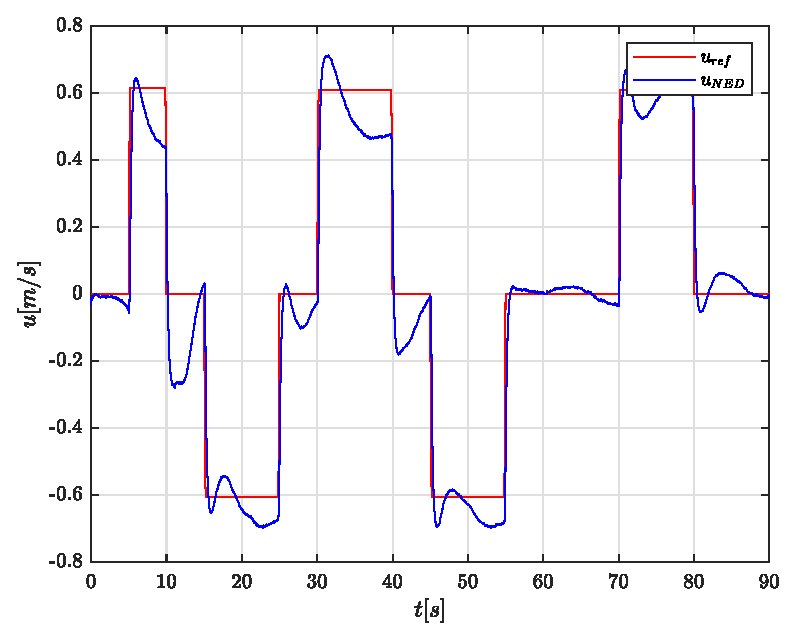
\includegraphics[width=1\textwidth]{Simulazioni/Figure/PID/SNAKE/PositionControlXVel}
		\caption{Controllo velocità lungo x}
		\label{fig:SNAKEerrvelxPID}
	\end{subfigure}
	\hfill
	\begin{subfigure}{0.45\textwidth}
		\centering
		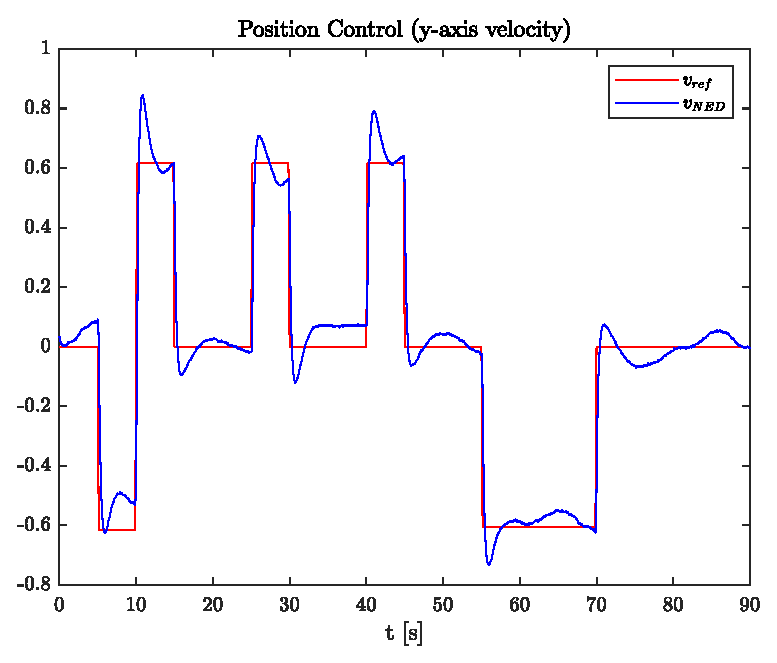
\includegraphics[width=1\textwidth]{Simulazioni/Figure/PID/SNAKE/PositionControlYVel}
		\caption{Controllo velocità lungo y}
		\label{fig:SNAKEerrvelyPID}
	\end{subfigure}
	\caption{Risposta in posizione con controllore interno PID al comando SNAKE}
\end{figure}

\begin{figure}
	\centering
	\begin{subfigure}{0.45\textwidth}
		\centering
		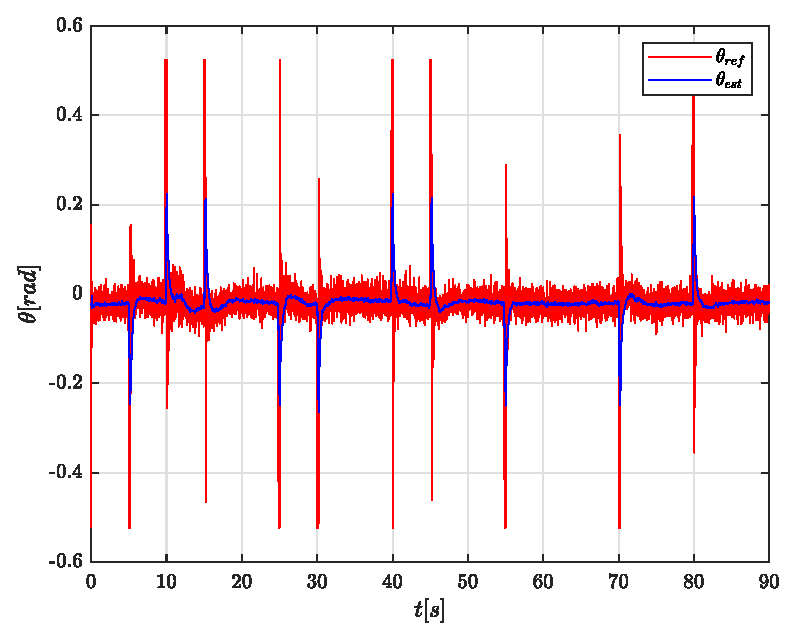
\includegraphics[width=1\textwidth]{Simulazioni/Figure/PID/SNAKE/AttitudeControlPitch}
		\caption{Controllo beccheggio}
		\label{fig:SNAKEerrbecPID}
	\end{subfigure}
	\hfill
	\begin{subfigure}{0.45\textwidth}
		\centering
		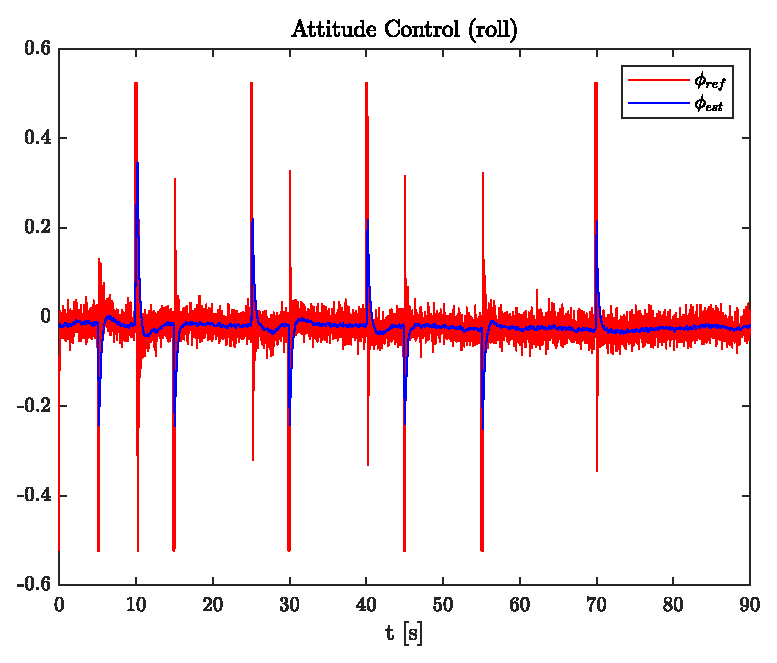
\includegraphics[width=1\textwidth]{Simulazioni/Figure/PID/SNAKE/AttitudeControlRoll}
		\caption{Controllo rollio}
		\label{fig:SNAKEerrrolPID}
	\end{subfigure}
	\hfill
	\begin{subfigure}{0.45\textwidth}
		\centering
		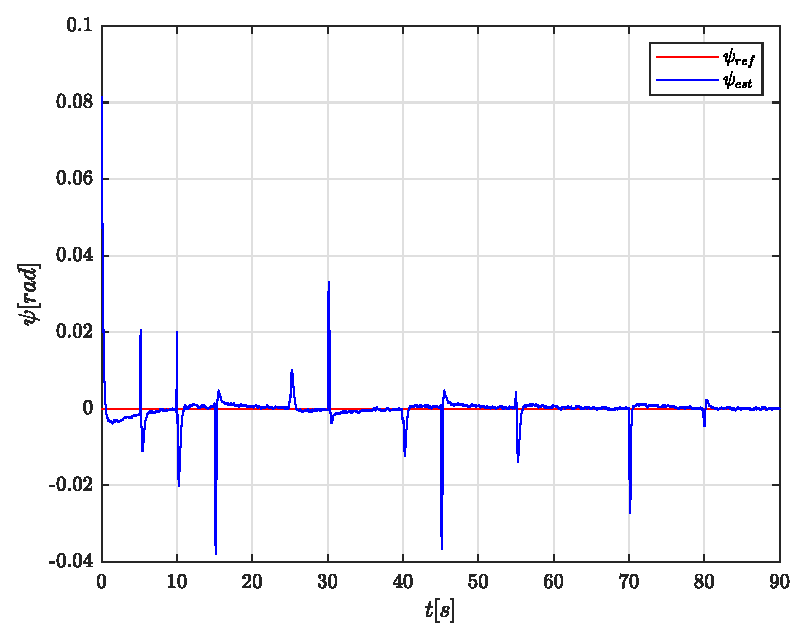
\includegraphics[width=1\textwidth]{Simulazioni/Figure/PID/SNAKE/AttitudeControlYaw}
		\caption{Controllo imbardata}
		\label{fig:SNAKEerryawPID}
	\end{subfigure}
	\caption{Risposta dell' assetto con controllore interno PID al comando SNAKE}
\end{figure}

\begin{figure}
	\centering
	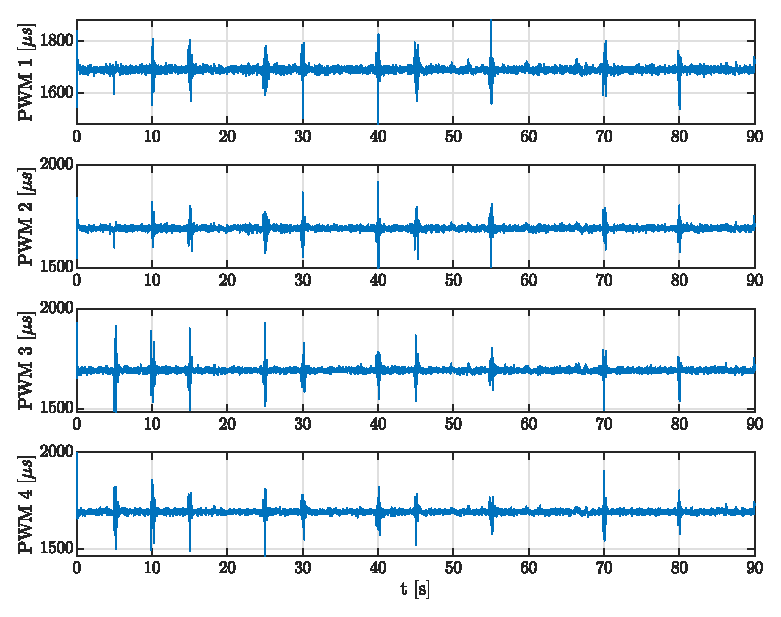
\includegraphics[width=0.5\textwidth]{Simulazioni/Figure/PID/SNAKE/PWM}
	\caption{Segnali PWM del controllore PID al segnale SNAKE}
	\label{fig:SNAKEPWMPID}
\end{figure}
\begin{figure}
	\centering
	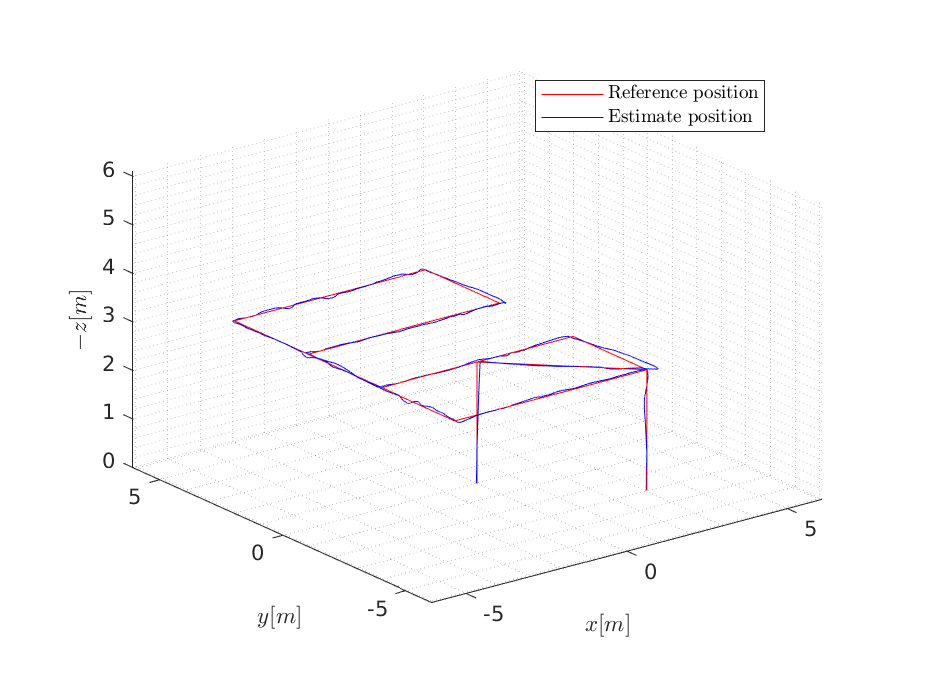
\includegraphics[width=1\textwidth]{Simulazioni/Figure/PID/SNAKE/Trajectory}
	\caption{Traiettoria percorsa con controllore PID al segnale SNAKE}
	\label{fig:SNAKEtraPID}
\end{figure}

In questa simulazione viene proposto un percorso più lungo in termine di tempo e spazio percorso. La risposta del sistema riguardante la posizione è precisa, presentando solo piccoli scostamenti nei punti in cui si ha una maggiore variazione di velocità, analogamente alle tre simulazioni mostrate in precedenza, Figure (\ref{fig:SNAKEerrposyPID}) e (\ref{fig:SNAKEerrposyPID}). Anche la risposta in termini di velocità a seguito di oscillazioni tende asintoticamente a rimanere nell'intorno del comando, Figure (\ref{fig:SNAKEerrposyPID}) e (\ref{fig:SNAKEerrposyPID}). Anche in questo caso i segnali di riferimento impartiti per gli angoli di beccheggio e rollio presentano delle situazioni di saturazione del cotnrollore di posizione e delle oscillazioni dovute alla presenza dei rumori dei sensori, Figure (\ref{fig:SNAKEerrbecPID}) e (\ref{fig:SNAKEerrrolPID}). La risposta del sistema rispetto all'angolo di imbardata è analogo alle simulazioni precedenti, Figura (\ref{fig:SNAKEerryawPID}). Il segnali PWM generati dal controllore non presentano particolari amplificazioni del rumore o saturazione, (\ref{fig:SNAKEPWMPID}). Osservando la traiettoria percorsa rispetto al riferimento, Figura (\ref{fig:SNAKEtraPID}), si nota l'efficacia del controllore con solo alcuni piccoli scostamenti.

\clearpage
\subsection{SMC}

Vengono qui riportate le simulazioni SIL utilizzando la configurazione denominata SMC nel capitolo \ref{cap:controllore}.

\subsubsection{STEP}


\begin{figure}
	\centering
	\begin{subfigure}{0.45\textwidth}
		\centering
		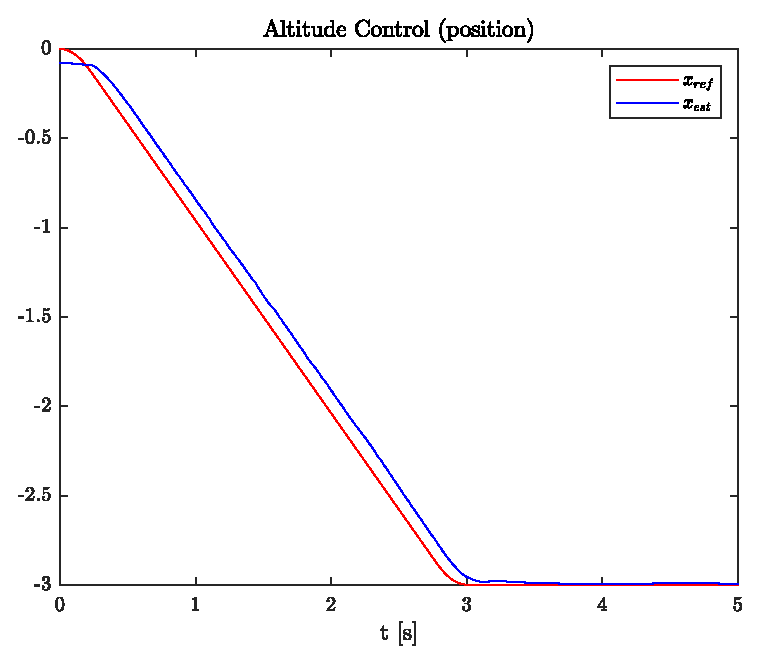
\includegraphics[width=1\textwidth]{Simulazioni/Figure/SMC/STEP/AltitudeControlPos}
		\caption{Controllo posizione}
		\label{fig:STEPerrposzSMC}
	\end{subfigure}
	\hfill
	\begin{subfigure}{0.45\textwidth}
		\centering
		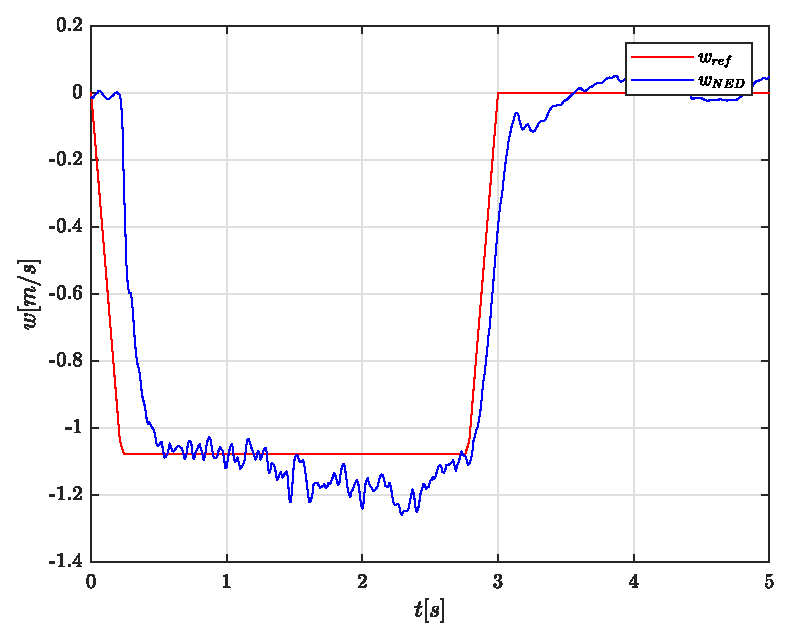
\includegraphics[width=1\textwidth]{Simulazioni/Figure/SMC/STEP/AltitudeControlVel}
		\caption{Controllo velocità}
		\label{fig:STEPerrvelzSMC}
	\end{subfigure}
	\caption{Risposta del controllore SMC di quota al segnale STEP}	
\end{figure}

\begin{figure}
	\centering
	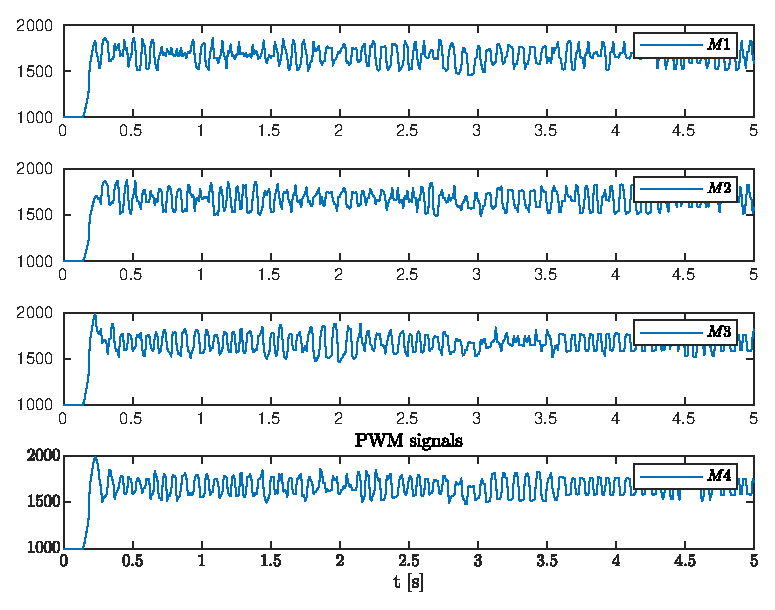
\includegraphics[width=0.5\textwidth]{Simulazioni/Figure/SMC/STEP/PWM}
	\caption{Segnali PWM generati del controllore SMC al segnale STEP}
	\label{fig:STEPPWMSMC}
\end{figure}

La risposta del controllore SMC in merito alla posizione è abbastanza precisa. Sussiste una differenza piccola ma costante lungo tutta la salita, differenza che si annulla rapidamente a livellamento, Figura (\ref{fig:STEPerrposzSMC}). Il profilo di velocità è seguito anch'esso con abbastanza precisione, esiste in questo caso un oscillazione costante nella risposta in velocità rispetto al valore di riferimento della velocità, Figura (\ref{fig:STEPerrvelzSMC}). Il segnale PWM generato da controllore mostra un comportamento discontinuo con ampiezza molto marcata, Figura (\ref{fig:STEPPWMSMC}).

\subsubsection{SQUARE}
\begin{figure}
	\centering
	\begin{subfigure}{0.45\textwidth}
		\centering
		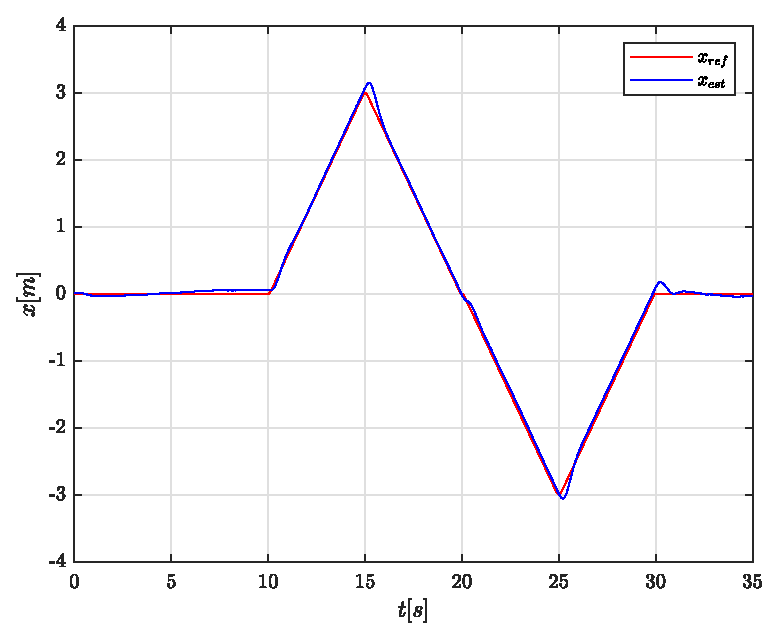
\includegraphics[width=1\textwidth]{Simulazioni/Figure/SMC/SQUARE/PositionControlXPos}
		\caption{Controllo posizione lungo x}
		\label{fig:SQUAREerrposxSMC}
	\end{subfigure}
	\hfill
	\begin{subfigure}{0.45\textwidth}
		\centering
		\includegraphics[width=1\textwidth]{Simulazioni/Figure/SMC/SQUARE/PositionControlYPos}
		\caption{Controllo posizione lungo y}
		\label{fig:SQUAREerrposySMC}
	\end{subfigure}
	\\
	\begin{subfigure}{0.45\textwidth}
		\centering
		\includegraphics[width=1\textwidth]{Simulazioni/Figure/SMC/SQUARE/PositionControlXVel}
		\caption{Controllo velocità lungo x}
		\label{fig:SQUAREerrvelxSMC}
	\end{subfigure}
	\hfill
	\begin{subfigure}{0.45\textwidth}
		\centering
		\includegraphics[width=1\textwidth]{Simulazioni/Figure/SMC/SQUARE/PositionControlYVel}
		\caption{Controllo velocità lungo y}
		\label{fig:SQUAREerrvelySMC}
	\end{subfigure}
	\caption{Risposta del controllo posizione con controllore SMC al comando SQUARE}
\end{figure}

\begin{figure}
	\centering
	\begin{subfigure}{0.45\textwidth}
		\centering
		\includegraphics[width=1\textwidth]{Simulazioni/Figure/SMC/SQUARE/AttitudeControlPitch}
		\caption{Controllo beccheggio}
		\label{fig:SQUAREbecSMC}
	\end{subfigure}
	\hfill
	\begin{subfigure}{0.45\textwidth}
		\centering
		\includegraphics[width=1\textwidth]{Simulazioni/Figure/SMC/SQUARE/AttitudeControlRoll}
		\caption{Controllo rollio}
		\label{fig:SQUARErolSMC}
	\end{subfigure}
	\hfill
	\begin{subfigure}{0.45\textwidth}
		\centering
		\includegraphics[width=1\textwidth]{Simulazioni/Figure/SMC/SQUARE/AttitudeControlYaw}
		\caption{Controllo imbardata}
		\label{fig:SQUAREyawSMC}
	\end{subfigure}
	\caption{Risposta dell' assetto con controllore interno SMC al comando SQUARE}
\end{figure}


\begin{figure}
	\centering
	\includegraphics[width=0.5\textwidth]{Simulazioni/Figure/SMC/SQUARE/PWM}
	\caption{Segnali PWM del controllore SMC al segnale SQUARE}
	\label{fig:SQUAREPWMSMC}
\end{figure}
\begin{figure}
	\centering
	\includegraphics[width=1\textwidth]{Simulazioni/Figure/SMC/SQUARE/Trajectory}
	\caption{Traiettoria percorsa con controllore SMC al segnale SQUARE}
	\label{fig:SQUAREtraSMC}
\end{figure}

\todo{Da cambiare}
In questa simulazione viene mostrata la capacità di muoversi nello spazio rispetto alle coordinate $x$ e $y$. L'errore di posizione osservato risulta essere relativamente piccolo. Gli incrementi di questo risultano essere maggiori nella fase di decollo iniziale e nell'attuazione dei cambi di velocità, Figure (\ref{fig:SQUAREerrposyPID}) e (\ref{fig:SQUAREerrposyPID}). L'inseguimento da parte del controllore PID nei confronti della velocità presenta alcuni picchi di overshoot quando questa subisce repentine variazioni, mostrando però l'assestamento successivo verso la riduzione asintotica della differenza. La risposta in velocità risulta essere molto rapida, Figure (\ref{fig:SQUAREerrvelyPID}) e (\ref{fig:SQUAREerrvelyPID}). Osservando i segnali di riferimento generati dal Position Control per l'Attitude Control,nelle Figure (\ref{fig:SQUAREerrbecPID}) e (\ref{fig:SQUAREerrrolPID}), si nota la presenza di intervalli in cui il controllore di posizione è in saturazione. Il segnale di riferimento generato dal Position Control presenta una componente di rumore. Il velivolo riesce comunque a seguire mediamente questo segnale, portandosi in condizione di assetto corretto per seguire la velocità di traslazione. Per quanto riguarda l'angolo di imbardata, con riferimento costante, presenta a causa degli effetti di accoppiamento tra le rotazioni lungo gli assi $x$ e $y$, degli scostamenti. Il sistema risponde molto bene per ridurre questo tipo di errore, come è osservabile nella Figura (\ref{fig:SQUAREerryawPID}). Anche in questa simulazione il segnale PWM generato è molto pulito e non presenta oscillazioni di ampiezza rilevante rispetto al valore medio, Figura (\ref{fig:SQUAREPWMPID}). Osservando la Figura (\ref{fig:SQUAREtraPID}), si osserva come il controllore sia in grado di percorrere la traiettoria prestabilita in modo efficacie, con alcune fasi di scostamento nelle variazione della direzione. La fase di atterraggio non presenta particolari criticità.


\subsubsection{BUTTERFLY}

\begin{figure}
	\centering
	\begin{subfigure}{0.45\textwidth}
		\centering
		\includegraphics[width=1\textwidth]{Simulazioni/Figure/SMC/BUTTERFLY/PositionControlXPos}
		\caption{Controllo posizione lungo x}
		\label{fig:BUTTERFLYerrposxSMC}
	\end{subfigure}
	\hfill
	\begin{subfigure}{0.45\textwidth}
		\centering
		\includegraphics[width=1\textwidth]{Simulazioni/Figure/SMC/BUTTERFLY/PositionControlYPos}
		\caption{Controllo posizione lungo y}
		\label{fig:BUTTERFLYerrposySMC}
	\end{subfigure}
	\\
	\begin{subfigure}{0.45\textwidth}
		\centering
		\includegraphics[width=1\textwidth]{Simulazioni/Figure/SMC/BUTTERFLY/PositionControlXVel}
		\caption{Controllo velocità lungo x}
		\label{fig:BUTTERFLYerrvelxSMC}
	\end{subfigure}
	\hfill
	\begin{subfigure}{0.45\textwidth}
		\centering
		\includegraphics[width=1\textwidth]{Simulazioni/Figure/SMC/BUTTERFLY/PositionControlYVel}
		\caption{Controllo velocità lungo y}
		\label{fig:BUTTERFLYerrvelySMC}
	\end{subfigure}
	\caption{Risposta in posizione con controllore interno SMC al comando BUTTERFLY}
\end{figure}

\begin{figure}
	\centering
	\begin{subfigure}{0.45\textwidth}
		\centering
		\includegraphics[width=1\textwidth]{Simulazioni/Figure/SMC/BUTTERFLY/AttitudeControlPitch}
		\caption{Controllo beccheggio}
		\label{fig:BUTTERFLYbecSMC}
	\end{subfigure}
	\hfill
	\begin{subfigure}{0.45\textwidth}
		\centering
		\includegraphics[width=1\textwidth]{Simulazioni/Figure/SMC/BUTTERFLY/AttitudeControlRoll}
		\caption{Controllo rollio}
		\label{fig:BUTTERFLYrolSMC}
	\end{subfigure}
	\hfill
	\begin{subfigure}{0.45\textwidth}
		\centering
		\includegraphics[width=1\textwidth]{Simulazioni/Figure/SMC/BUTTERFLY/AttitudeControlYaw}
		\caption{Controllo imbardata}
		\label{fig:BUTTERFLYyawSMC}
	\end{subfigure}
	\caption{Risposta dell' assetto con controllore interno SMC al comando BUTTERFLY}
\end{figure}

\begin{figure}
	\centering
	\includegraphics[width=0.5\textwidth]{Simulazioni/Figure/SMC/BUTTERFLY/PWM}
	\caption{Segnali PWM del controllore SMC al segnale BUTTERFLY}
	\label{fig:BUTTERFLYPWMSMC}
\end{figure}
\begin{figure}
	\centering
	\includegraphics[width=1\textwidth]{Simulazioni/Figure/SMC/BUTTERFLY/Trajectory}
	\caption{Traiettoria percorsa con controllore SMC al segnale BUTTERFLY}
	\label{fig:BUTTERFLYtraSMC}
\end{figure}

\todo{Da cambiare}
In questa simulazione si oserva come il controllore PID risponda correttamente al comando di decollo. L'errore iniziale risulta essere maggiore nella prima fase a causa dell'errore misurato inizialmente sulla quota. Nel proseguire della manovra il sistema riesce correttamente a minimizzare corettamente l'errore di posizione, Figura (\ref{fig:STEPerrposzPID}). L'inseguimento del rateo di salita risulta essere imprecisa nella fase iniziale, presentando un overshoot e un successivo assestamento lento è impreciso. Nella fase di livellamento però sia l'overshoot che l'errore stazionario si riduce, Figura (\ref{fig:STEPerrposzPID}). Il segnale PWM in uscita del controllore risulta essere abbastanza regolare, senza presentare oscillazioni eccessive, rimanendo in un range nominale e non presentando saturazione.

\subsubsection{SNAKE}
\begin{figure}
	\centering
	\begin{subfigure}{0.45\textwidth}
		\centering
		\includegraphics[width=1\textwidth]{Simulazioni/Figure/SMC/SNAKE/PositionControlXPos}
		\caption{Controllo posizione lungo x}
		\label{fig:SNAKEerrposxSMC}
	\end{subfigure}
	\hfill
	\begin{subfigure}{0.45\textwidth}
		\centering
		\includegraphics[width=1\textwidth]{Simulazioni/Figure/SMC/SNAKE/PositionControlYPos}
		\caption{Controllo posizione lungo y}
		\label{fig:SNAKEerrposySMC}
	\end{subfigure}
	\\
	\begin{subfigure}{0.45\textwidth}
		\centering
		\includegraphics[width=1\textwidth]{Simulazioni/Figure/SMC/SNAKE/PositionControlXVel}
		\caption{Controllo velocità lungo x}
		\label{fig:SNAKEerrvelxSMC}
	\end{subfigure}
	\hfill
	\begin{subfigure}{0.45\textwidth}
		\centering
		\includegraphics[width=1\textwidth]{Simulazioni/Figure/SMC/SNAKE/PositionControlYVel}
		\caption{Controllo velocità lungo y}
		\label{fig:SNAKEerrvelySMC}
	\end{subfigure}
	\caption{Risposta in posizione con controllore interno SMC al comando SNAKE}
\end{figure}

\begin{figure}
	\centering
	\begin{subfigure}{0.45\textwidth}
		\centering
		\includegraphics[width=1\textwidth]{Simulazioni/Figure/SMC/SNAKE/AttitudeControlPitch}
		\caption{Controllo beccheggio}
		\label{fig:SNAKEbecSMC}
	\end{subfigure}
	\hfill
	\begin{subfigure}{0.45\textwidth}
		\centering
		\includegraphics[width=1\textwidth]{Simulazioni/Figure/SMC/SNAKE/AttitudeControlRoll}
		\caption{Controllo rollio}
		\label{fig:SNAKErolSMC}
	\end{subfigure}
	\hfill
	\begin{subfigure}{0.45\textwidth}
		\centering
		\includegraphics[width=1\textwidth]{Simulazioni/Figure/SMC/SNAKE/AttitudeControlYaw}
		\caption{Controllo imbardata}
		\label{fig:SNAKEyawSMC}
	\end{subfigure}
	\caption{Risposta dell' assetto con controllore interno SMC al comando SNAKE}
\end{figure}


\begin{figure}
	\centering
	\includegraphics[width=0.5\textwidth]{Simulazioni/Figure/SMC/SNAKE/PWM}
	\caption{Segnali PWM del controllore SMC al segnale SNAKE}
	\label{fig:SNAKEPWMSMC}
\end{figure}
\begin{figure}
	\centering
	\includegraphics[width=1\textwidth]{Simulazioni/Figure/SMC/SNAKE/Trajectory}
	\caption{Traiettoria percorsa con controllore SMC al segnale SNAKE}
	\label{fig:SNAKEtraSMC}
\end{figure}

\todo{Da cambiare}
In questa simulazione viene mostrata la capacità di muoversi nello spazio rispetto alle coordinate $x$ e $y$. L'errore di posizione osservato risulta essere relativamente piccolo. Gli incrementi di questo risultano essere maggiori nella fase di decollo iniziale e nell'attuazione dei cambi di velocità, Figure (\ref{fig:SQUAREerrposyPID}) e (\ref{fig:SQUAREerrposyPID}). L'inseguimento da parte del controllore PID nei confronti della velocità presenta alcuni picchi di overshoot quando questa subisce repentine variazioni, mostrando però l'assestamento successivo verso la riduzione asintotica della differenza. La risposta in velocità risulta essere molto rapida, Figure (\ref{fig:SQUAREerrvelyPID}) e (\ref{fig:SQUAREerrvelyPID}). Osservando i segnali di riferimento generati dal Position Control per l'Attitude Control,nelle Figure (\ref{fig:SQUAREerrbecPID}) e (\ref{fig:SQUAREerrrolPID}), si nota la presenza di intervalli in cui il controllore di posizione è in saturazione. Il segnale di riferimento generato dal Position Control presenta una componente di rumore. Il velivolo riesce comunque a seguire mediamente questo segnale, portandosi in condizione di assetto corretto per seguire la velocità di traslazione. Per quanto riguarda l'angolo di imbardata, con riferimento costante, presenta a causa degli effetti di accoppiamento tra le rotazioni lungo gli assi $x$ e $y$, degli scostamenti. Il sistema risponde molto bene per ridurre questo tipo di errore, come è osservabile nella Figura (\ref{fig:SQUAREerryawPID}). Anche in questa simulazione il segnale PWM generato è molto pulito e non presenta oscillazioni di ampiezza rilevante rispetto al valore medio, Figura (\ref{fig:SQUAREPWMPID}). Osservando la Figura (\ref{fig:SQUAREtraPID}), si osserva come il controllore sia in grado di percorrere la traiettoria prestabilita in modo efficacie, con alcune fasi di scostamento nelle variazione della direzione. La fase di atterraggio non presenta particolari criticità.

\subsection{Confronto}
\todo[inline]{Descrizione della precisione maggiore del SMC rispetto al PID a discapito del consumo maggiore}
	\section{Simulazioni PIL}
\todo[inline]{Descrizione del metodo di collegamento}
\todo[inline]{Parlare dell'importanza dello script di boot e fare riferimento all'appendice}
\todo[inline]{Descrizione dei successi e fallimenti nella simulazione}
\todo[inline]{Input correttamente comunicati dal simulatore}
\todo[inline]{Problema con gli output non comunicati al simulatore}

	\subsection{Conclusione}
\todo[inline]{Sviluppi futuri}


 %lavori futuri
	
	\backmatter
	\chapter{Appendice}
\subsection{Gazebo}

\lstset{language=c++}
\begin{lstlisting}
//gazebo_motor_model.cpp

...

//Leggo i parametri dal file di impostazione

getSdfParam<double>(_sdf, "ForceQuadraticCoefficent", force_quadratic_coefficent_, force_quadratic_coefficent_);
getSdfParam<double>(_sdf, "ForceLinearCoefficent", force_linear_coefficent_, force_linear_coefficent_);
getSdfParam<double>(_sdf, "ForceCostant", force_costant_, force_costant_);
getSdfParam<double>(_sdf, "ForceMinRpmFitting", force_min_rpm_fitting_, force_min_rpm_fitting_);

getSdfParam<double>(_sdf, "MomentQuadraticCoefficent", moment_quadratic_coefficent_, moment_quadratic_coefficent_);
getSdfParam<double>(_sdf, "MomentLinearCoefficent", moment_linear_coefficent_, moment_linear_coefficent_);
getSdfParam<double>(_sdf, "MomentCostant", moment_costant_, moment_costant_);
getSdfParam<double>(_sdf, "MomentMinRpmFitting", moment_min_rpm_fitting_, moment_min_rpm_fitting_);

...

//Aggiungo modifica forma quadratica
double force = std::isgreater(std::abs(real_motor_velocity),force_min_rpm_fitting_)*
(real_motor_velocity * real_motor_velocity * force_quadratic_coefficent_ 
+ std::abs(real_motor_velocity)* force_linear_coefficent_ + force_costant_);
if (force<0) force=0;

link_->AddRelativeForce(ignition::math::Vector3d(0, 0, force));

ignition::math::Vector3d drag_torque(0, 0, -turning_direction_ *
std::isgreater(std::abs(real_motor_velocity),
moment_min_rpm_fitting_)*(real_motor_velocity * 
real_motor_velocity * moment_quadratic_coefficent_ + 
std::abs(real_motor_velocity) * moment_linear_coefficent_+ moment_costant_));

...

ignition::math::Vector3d drag_torque_parent_frame = pose_difference.Rot().RotateVector(drag_torque);
parent_links.at(0)->AddRelativeTorque(drag_torque_parent_frame);

...

\end{lstlisting}

\lstset{language=XML}
\begin{lstlisting}
<!-- drone.sdf-->

...

<plugin name='front_left_motor_model' filename='libgazebo_motor_model.so'>
<robotNamespace/>
<jointName>rotor_3_joint</jointName>
<linkName>rotor_3</linkName>
<turningDirection>cw</turningDirection>
<maxRotVelocity>2000</maxRotVelocity>
<commandSubTopic>/gazebo/command/motor_speed</commandSubTopic>
<motorNumber>3</motorNumber>
<motorSpeedPubTopic>/motor_speed/3</motorSpeedPubTopic>
<rotorVelocitySlowdownSim>10</rotorVelocitySlowdownSim>
<ForceQuadraticCoefficent>1.1632e-5</ForceQuadraticCoefficent>
<ForceLinearCoefficent>-0.0202</ForceLinearCoefficent>
<ForceCostant>8.1513</ForceCostant>
<ForceMinRpmFitting>1000</ForceMinRpmFitting>
<MomentQuadraticCoefficent>2.6604e-7</MomentQuadraticCoefficent>
<MomentLinearCoefficent>-4.6797e-4</MomentLinearCoefficent>
<MomentCostant>0.2046</MomentCostant>
<MomentMinRpmFitting>1000</MomentMinRpmFitting>

...

\end{lstlisting}
	\nocite{*}
\printbibliography[heading=bibintoc]
	
\end{document}